\chapter[Pruebas y resultados experimentales]{ Pruebas y resultados experimentales}
\pagestyle{fancy}

En este cap\'itulo se abordar\'a los resultados obtenidos a fin de dar cumplimiento de los objetivos definidos en este TFG, adem\'as de verificación del correcto funcionamiento del sistema dise\~nado, mediantes los reportes y an\'alisis de datos obtenidos a partir de las  pruebas de funcionamiento en ambientes controlados y pruebas de campo en el Lago Ypakarai.  As\'i mismo  las configuraciones correspondientes a fin de obtener las lecturas en tiempo real en la estaci\'on remota, ubicada en la sala de monitoreo del laboratorio de sistemas. distribuido (LSD) en CITEC.
\section{Prueba en ambientes controlados}
Las pruebas en ambientes controlados, consisti\'o en una serie de pruebas realizados en el laboratorio de sistemas distribuido y en el laboratorio de qu\'imica, a fin de poner a punto todos los elementos que conforman el sistema a ser desplegados, antes de realizar las pruebas en campo, donde se espera que se encuentren m\'as variables a tener en cuenta, que deben prever y probar con anticipaci\'on de tal forma de evitar menos fallas.
En este efecto, en este apartado se abarcar\'an los trabajos realizados para la puesta a punto de los sensores Atlas Scientific.

\subsection{Calibraciones de sensores}
La calibraci\'on de los sensores, es fundamental para que pueda representar una lectura correcta de los valores a ser medidos, a este efecto los sensores adquiridos para la sonda, fueron prove\'idos en un kit que se puede observar en la figura \ref{fig:kit}, los cuales inclu\'ian l\'iquidos de calibraci\'on para cada uno de los sensores adquiridos. 

El kit de l\'iquidos de calibraciones est\'a compuesta un total de ocho botellas, de las cuales una de ellas contiene un l\'iquido de almacenamiento. Cada sensor posee un tipo de calibraci\'on distinta, que var\'ia seg\'un la cantidad de puntos que requiere para ajustar la curva de lectura de mediciones.
El caso del sensor de pH requiere de tres puntos de calibración (bajo, medio y alto), para los cuales se utiliza pH=4 para la calibraci\'on del punto bajo, pH=7 para la calibraci\'on del punto medio y pH=10 para la calibraci\'on del punto alto, con estas 3 calibraciones el sensor de pH se encuentra listo.
El sensor de OD, requiere dos puntos de calibraci\'on, la primera calibraci\'on que consiste en la calibraci\'on a los niveles de ox\'igeno atmosf\'erico y el segundo con su l\'iquido test correspondiente.
El sensor de OPR, solo requiere un valor conocido de OPR para su calibraci\'on, para su efecto se utiliza el l\'iquido de calibraci\'on que posee un valor de 225 mV.
El sensor de conductividad el\'ectrica, requiere de dos puntos de calibraci\'on (alto y bajo), para los cuales se utilizaron CE=12.880 $\mu S/cm$ para la calibraci\'on del punto bajo y CE=80.000 $\mu S/cm$ para la calibraci\'on del punto alto.

La calibraci\'on se realiza, con la sobrescritura del valor de lectura muestreado al l\'iquido de calibraci\'on, con el valor esperado seg\'un los datos proporcionados, mediante protocolo de comunicaci\'on i2C o serial, a la placa driver del sensor, con el comando \textbf{CAL,n }, donde CAL es el comando de calibraci\'on y n el valor a ser sobrescrito.
\begin{figure}[H]
        \centering
        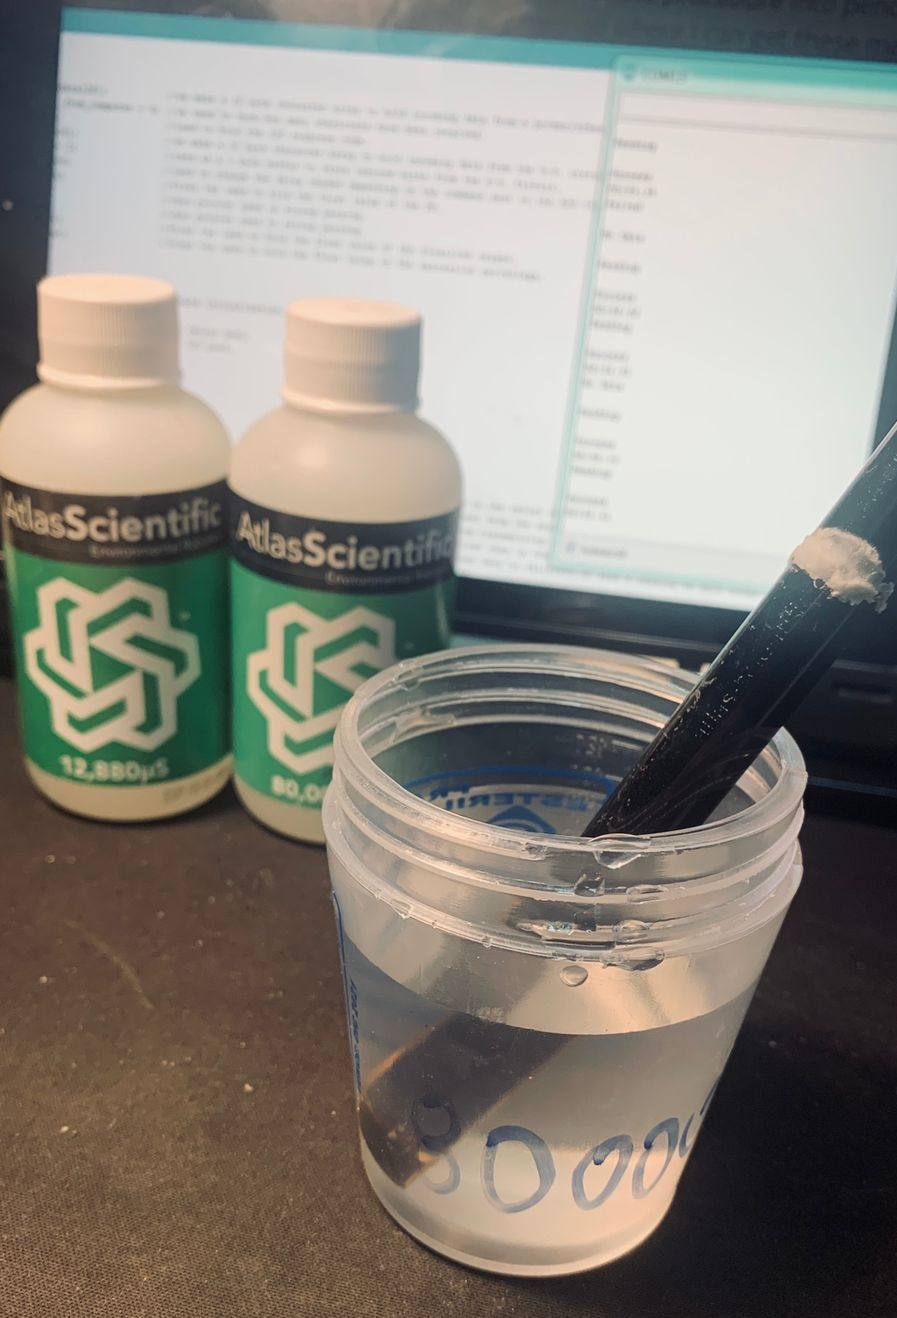
\includegraphics[scale=0.5]{Imagenes/cap4/calibracion.jpeg}
        \caption {Calibraci\'on sensor CE. }{\textbf{Fuente:}
        Elaboraci\'on propia}
        \label{fig:kit}
\end{figure}
Los sensores se consideran calibrados, si pueden realizar lecturas sobre l\'iquidos cuyos valores sean conocidos con un dentro del error esperado o previsto por el fabricante, en el caso de no conseguir una lectura correcta, se debe de borrar las configuraciones de calibraci\'on con el comando \textbf{Cal, clear} y volver a realizar el procedimiento anterior, una vez limpiado todos los equipos utilizados a fin de equipar contaminación. 
En el caso de los sensores de pH y OPR, se deben almacenar con su l\'iquido de almacenamiento.
\subsection{Muestreo en el laboratorio qu\'imica - FIUNA }
El monitoreo se realiz\'o en el laboratorio de qu\'imica de la facultad de ingenier\'ia de la Universidad Nacional de Asunci\'on [QCA], sede San Lorenzo, de los par\'ametros temperatura[T], conductividad el\'ectrica[CE], potencial de hidr\'ogeno[pH]. A fin de poder contrastar los sensores utilizados con los sensores disponibles en el laboratorio de qu\'imica.


\subsubsection{Metodolog\'ia }
La metodolog\'ia de recolección y muestreo consisti\'o en el an\'alisis de tres tipos de muestras distintas, la muestra 1 consisti\'o en agua doble destilada, la muestra 2 consisti\'o en agua de pozo, obtenida de una de las redes de abastecimiento de la zona del campus universitario y la muestra 3 consisti\'o en agua de laguna obtenida en la Facultad de Ciencias Exactas y Naturales (FACEN). Cada una de estas muestras se dividieron equitativamente en tres recipientes distintos, de tal forma de obtener el mismo l\'iquido en tres recientes que ser\'an muestreado y registrado las primeras 5 lecturas estables con el multisensor del laboratorio de qu\'imica e igual n\'umero de veces con los sensores de la sonda disen\~nada.
Los par\'ametros a ser analizados en este apartado son pH, CE y T, por la disponibilidad en ese momento de los equipos.
Las caracter\'isticas de los sensores del laboratorio de qu\'imica utilizados se pueden visualizar en la tabla \ref{tab: Sensores laboratorio de quimica}
Sensores laboratorio de qu\'imica, las caracter\'isticas de los otros sensores se encuentran en el cap\'itulo 2, correspondientes al sensor de CE,T,Ph de la empresa Atlas Scientific.
\begin{table}[H]
    \caption{Caracter\'isticas de los sensores de laboratorio de qu\'imica}
    \label{tab: Sensores laboratorio de quimica}
    \begin{tabular}{l c c}
        \toprule
        Caracter\'isticas & Sensor $pH$ & Sensor  $CE$ \\
        \midrule
        Marca & Ohaus       & Oaklon       \\
        Serie & ST10        & WD-35462-11  \\
        Intervalo de medici\'on                      & 0.00 – 14 {[}pH{]} & 0.00 – 20.00 {[}mS/cm{]}        \\
        Resoluci\'on de la medici\'on & 0.1   {[}pH{]}     & TDS 10 {[}ppm{]}, 0,1 {[}ppt{]} \\
        Precisi\'on                                  & $\pm0,1$ {[}pH{]}  & $\pm0,1$ {[}mS/cm{]}   
    \end{tabular}
 \end{table}
Las lecturas se realizaron de forma secuencial con ambos sensores, figura \ref{fig: Muestreo de CE}, cada vez que terminaba el muestreo en cada uno de el recipiente con una de la muestras, se proced\'ia registrar la lectura estable obtenida, retirar el sensor utilizado, limpiarlo con agua destilada y secar con un pa\~no, e introducir el otro sensor equivalente para repetir el procedimiento hasta completar los cinco muestreos.

\begin{figure}
     \centering
     \begin{subfigure}[b]{0.25\textwidth}
         \centering
         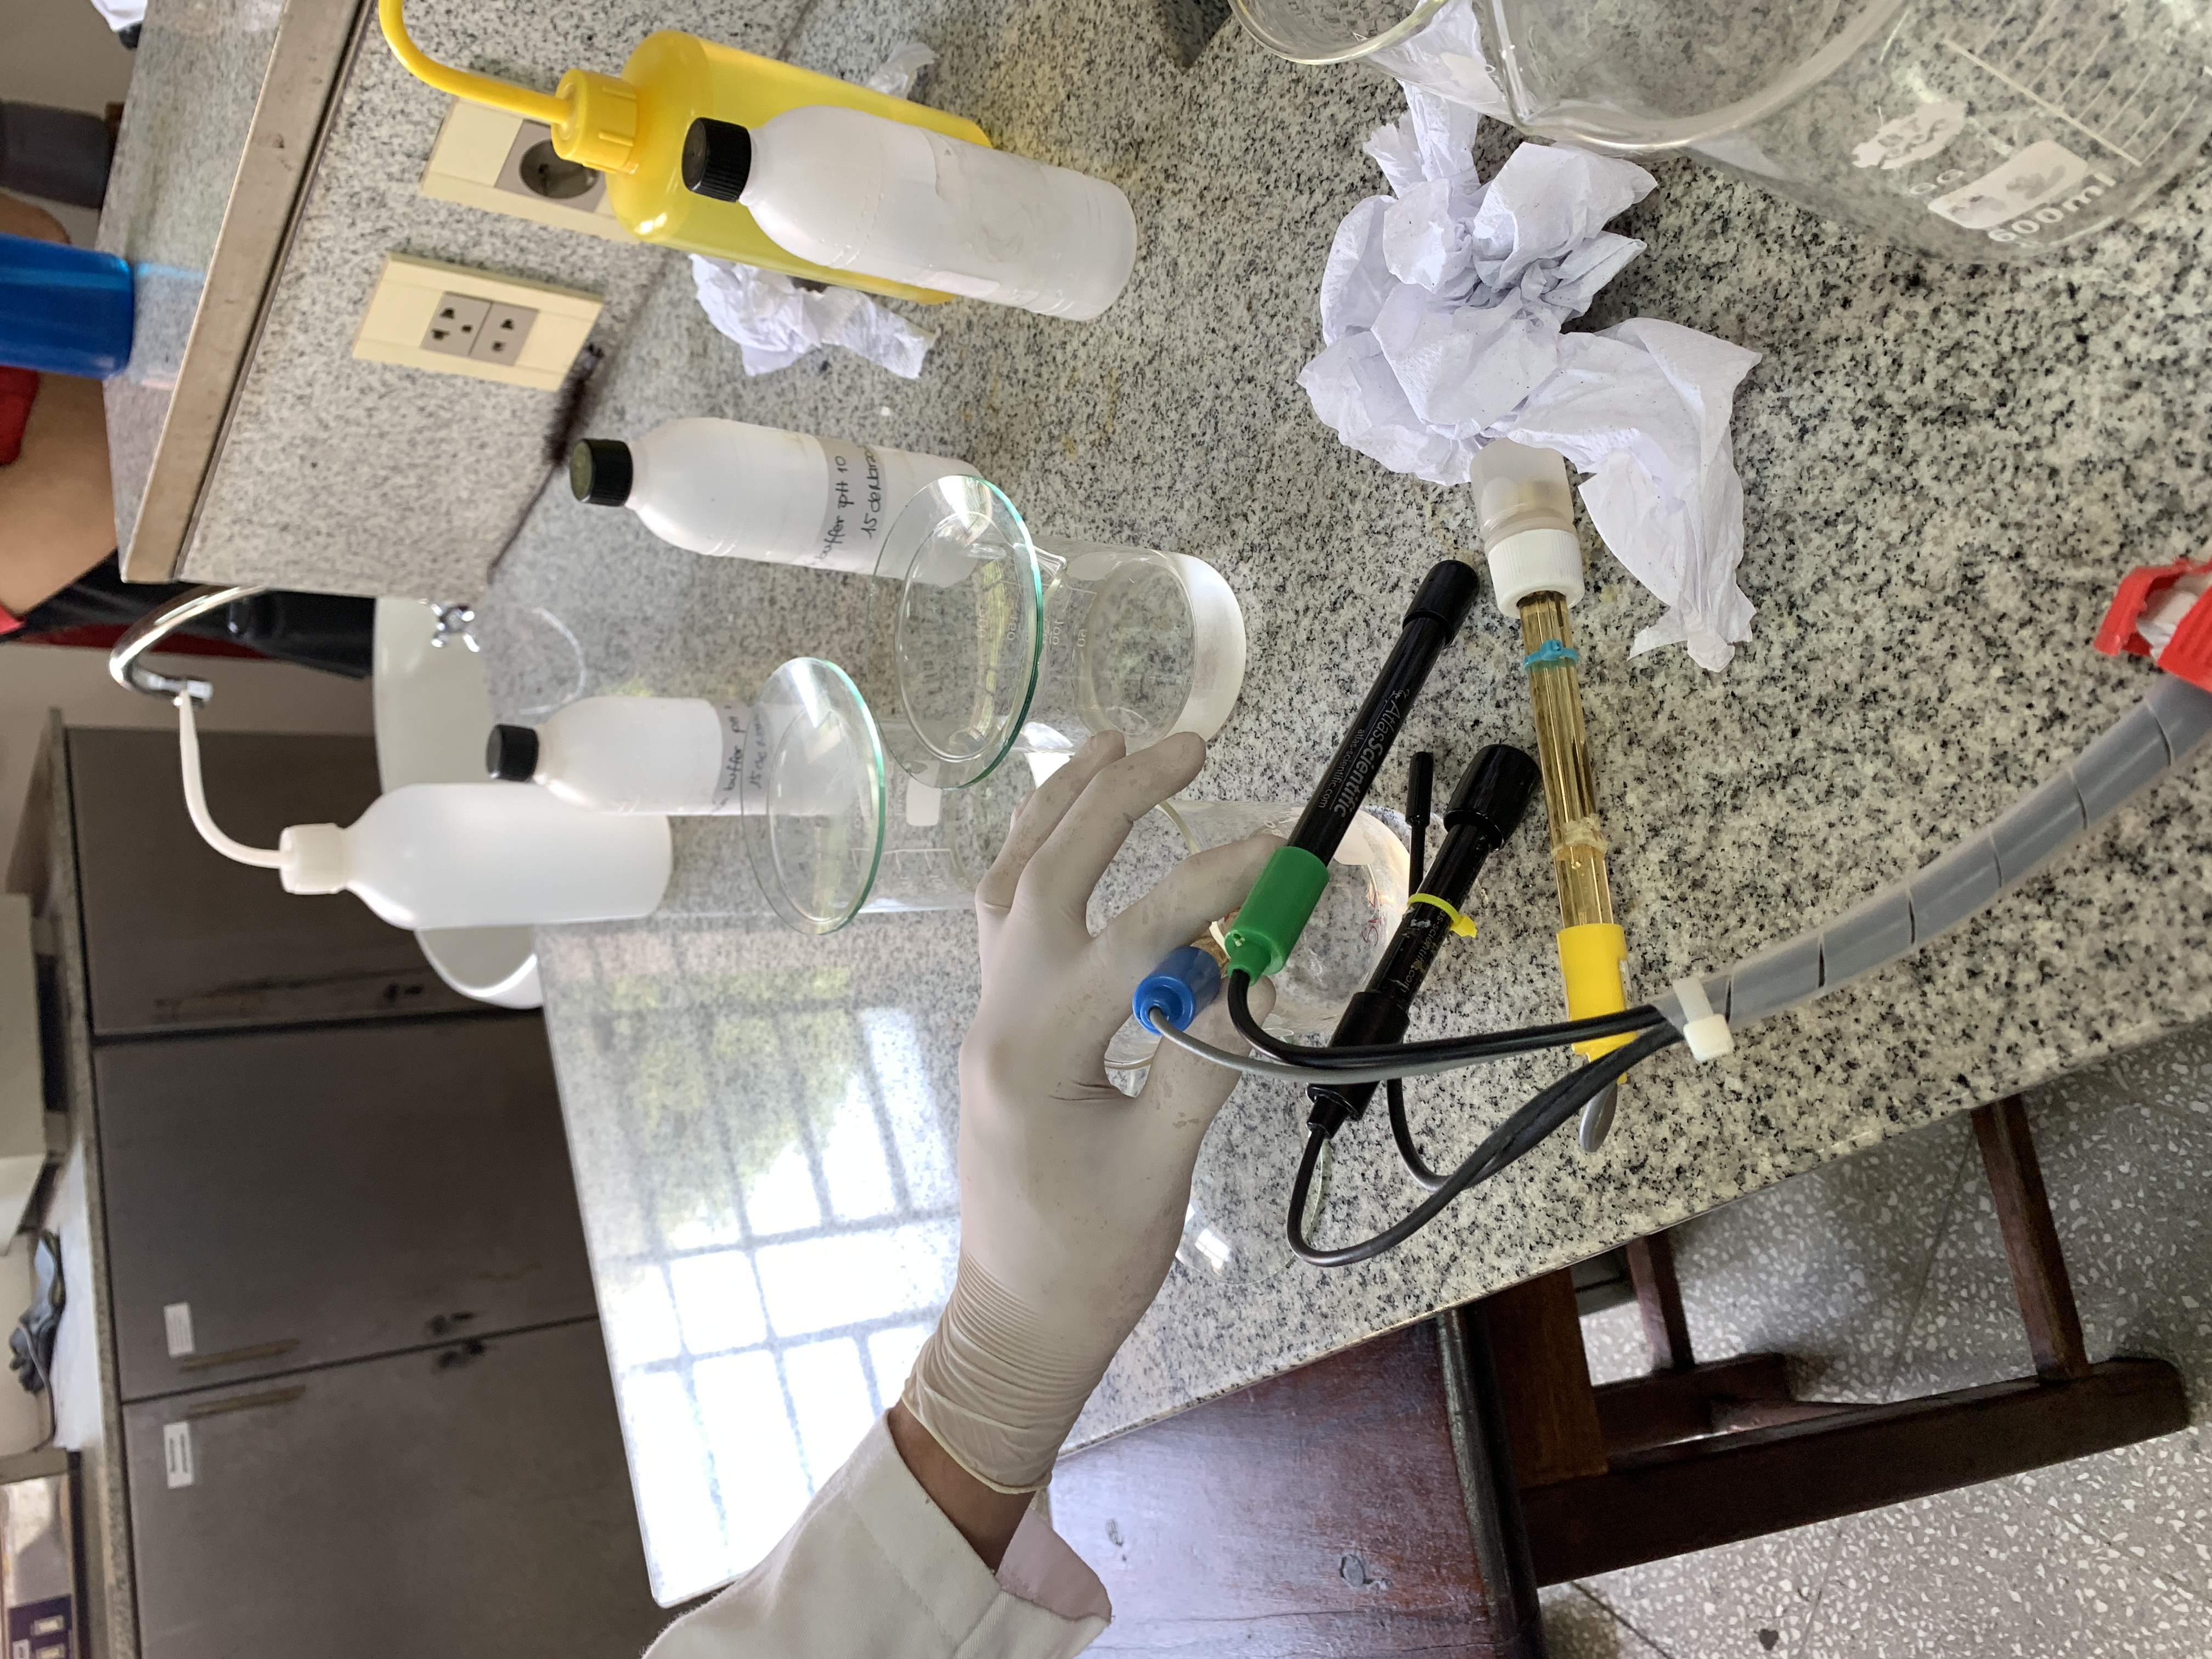
\includegraphics[angle=270,width=\textwidth]{Imagenes/cap4/qca1.jpg}
         \caption{Sensores sonda.}
         \label{fig:calibracionLSD}
     \end{subfigure}
     \hfill
     \begin{subfigure}[b]{0.4\textwidth}
         \centering
         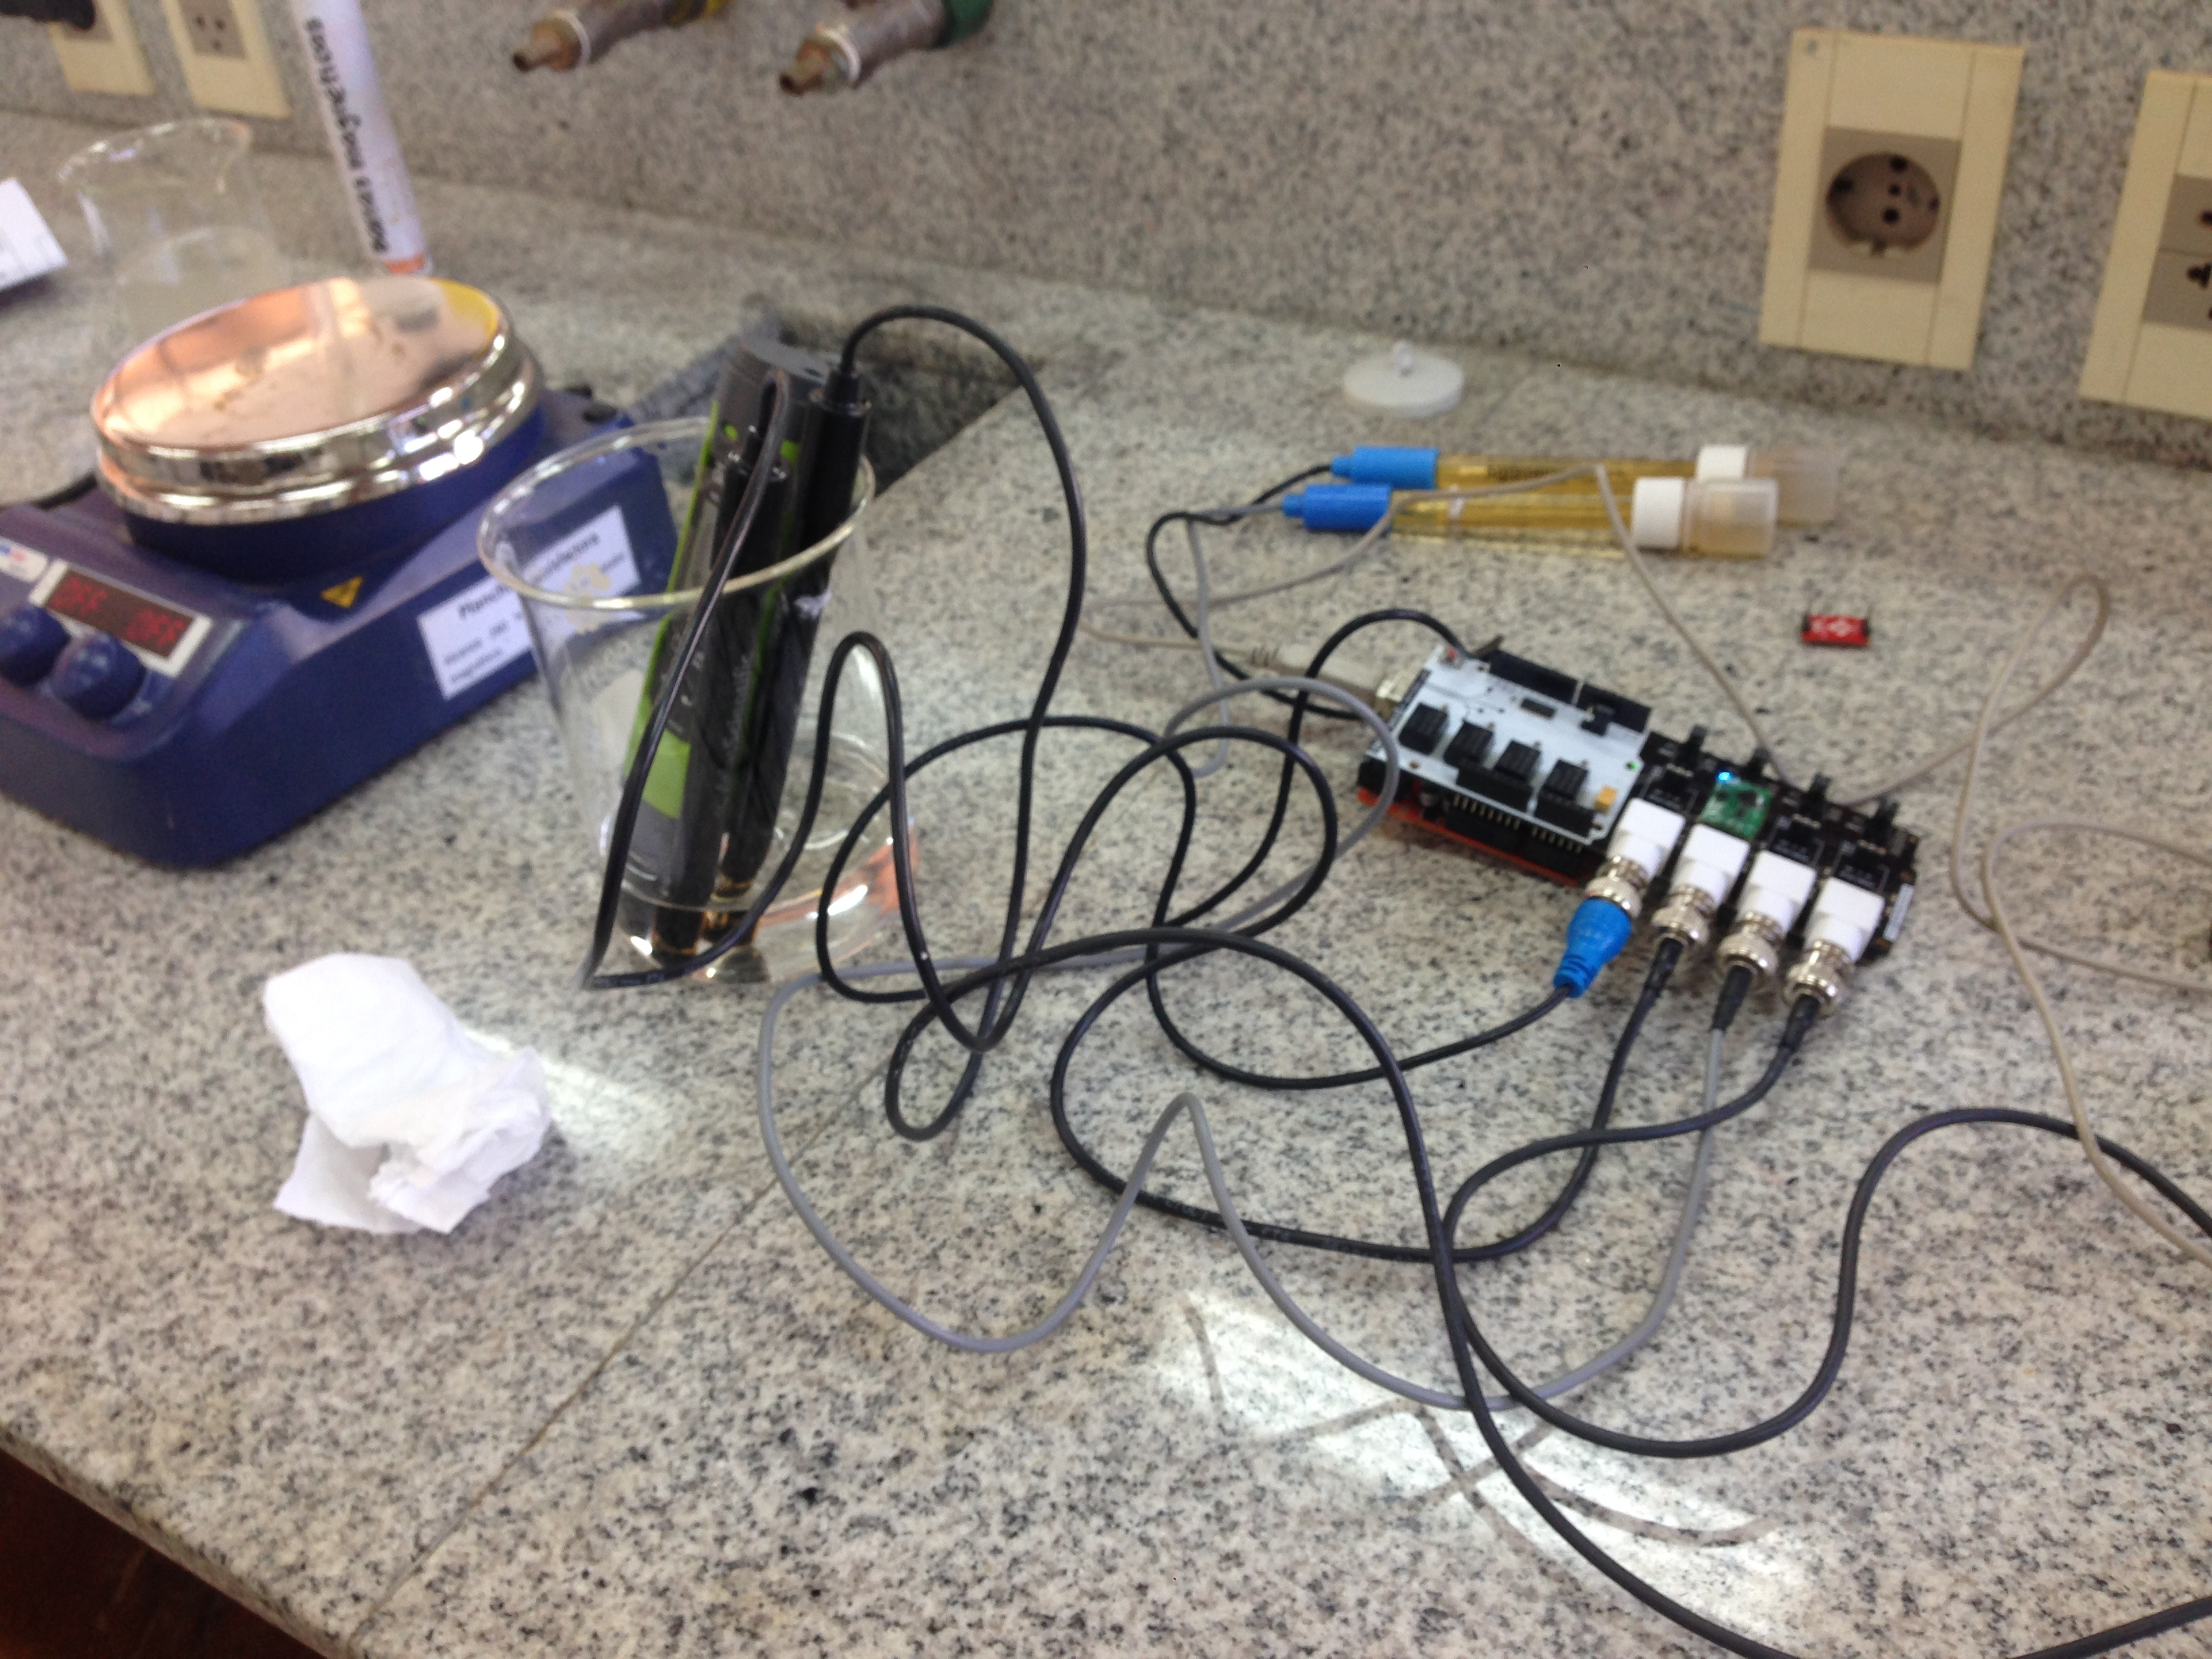
\includegraphics[width=\textwidth]{Imagenes/cap4/qca2.jpg}
         \caption{Placa de sensores}
         \label{fig:placas_muestreo}
     \end{subfigure}
     \hfill
     \begin{subfigure}[b]{0.25\textwidth}
         \centering
         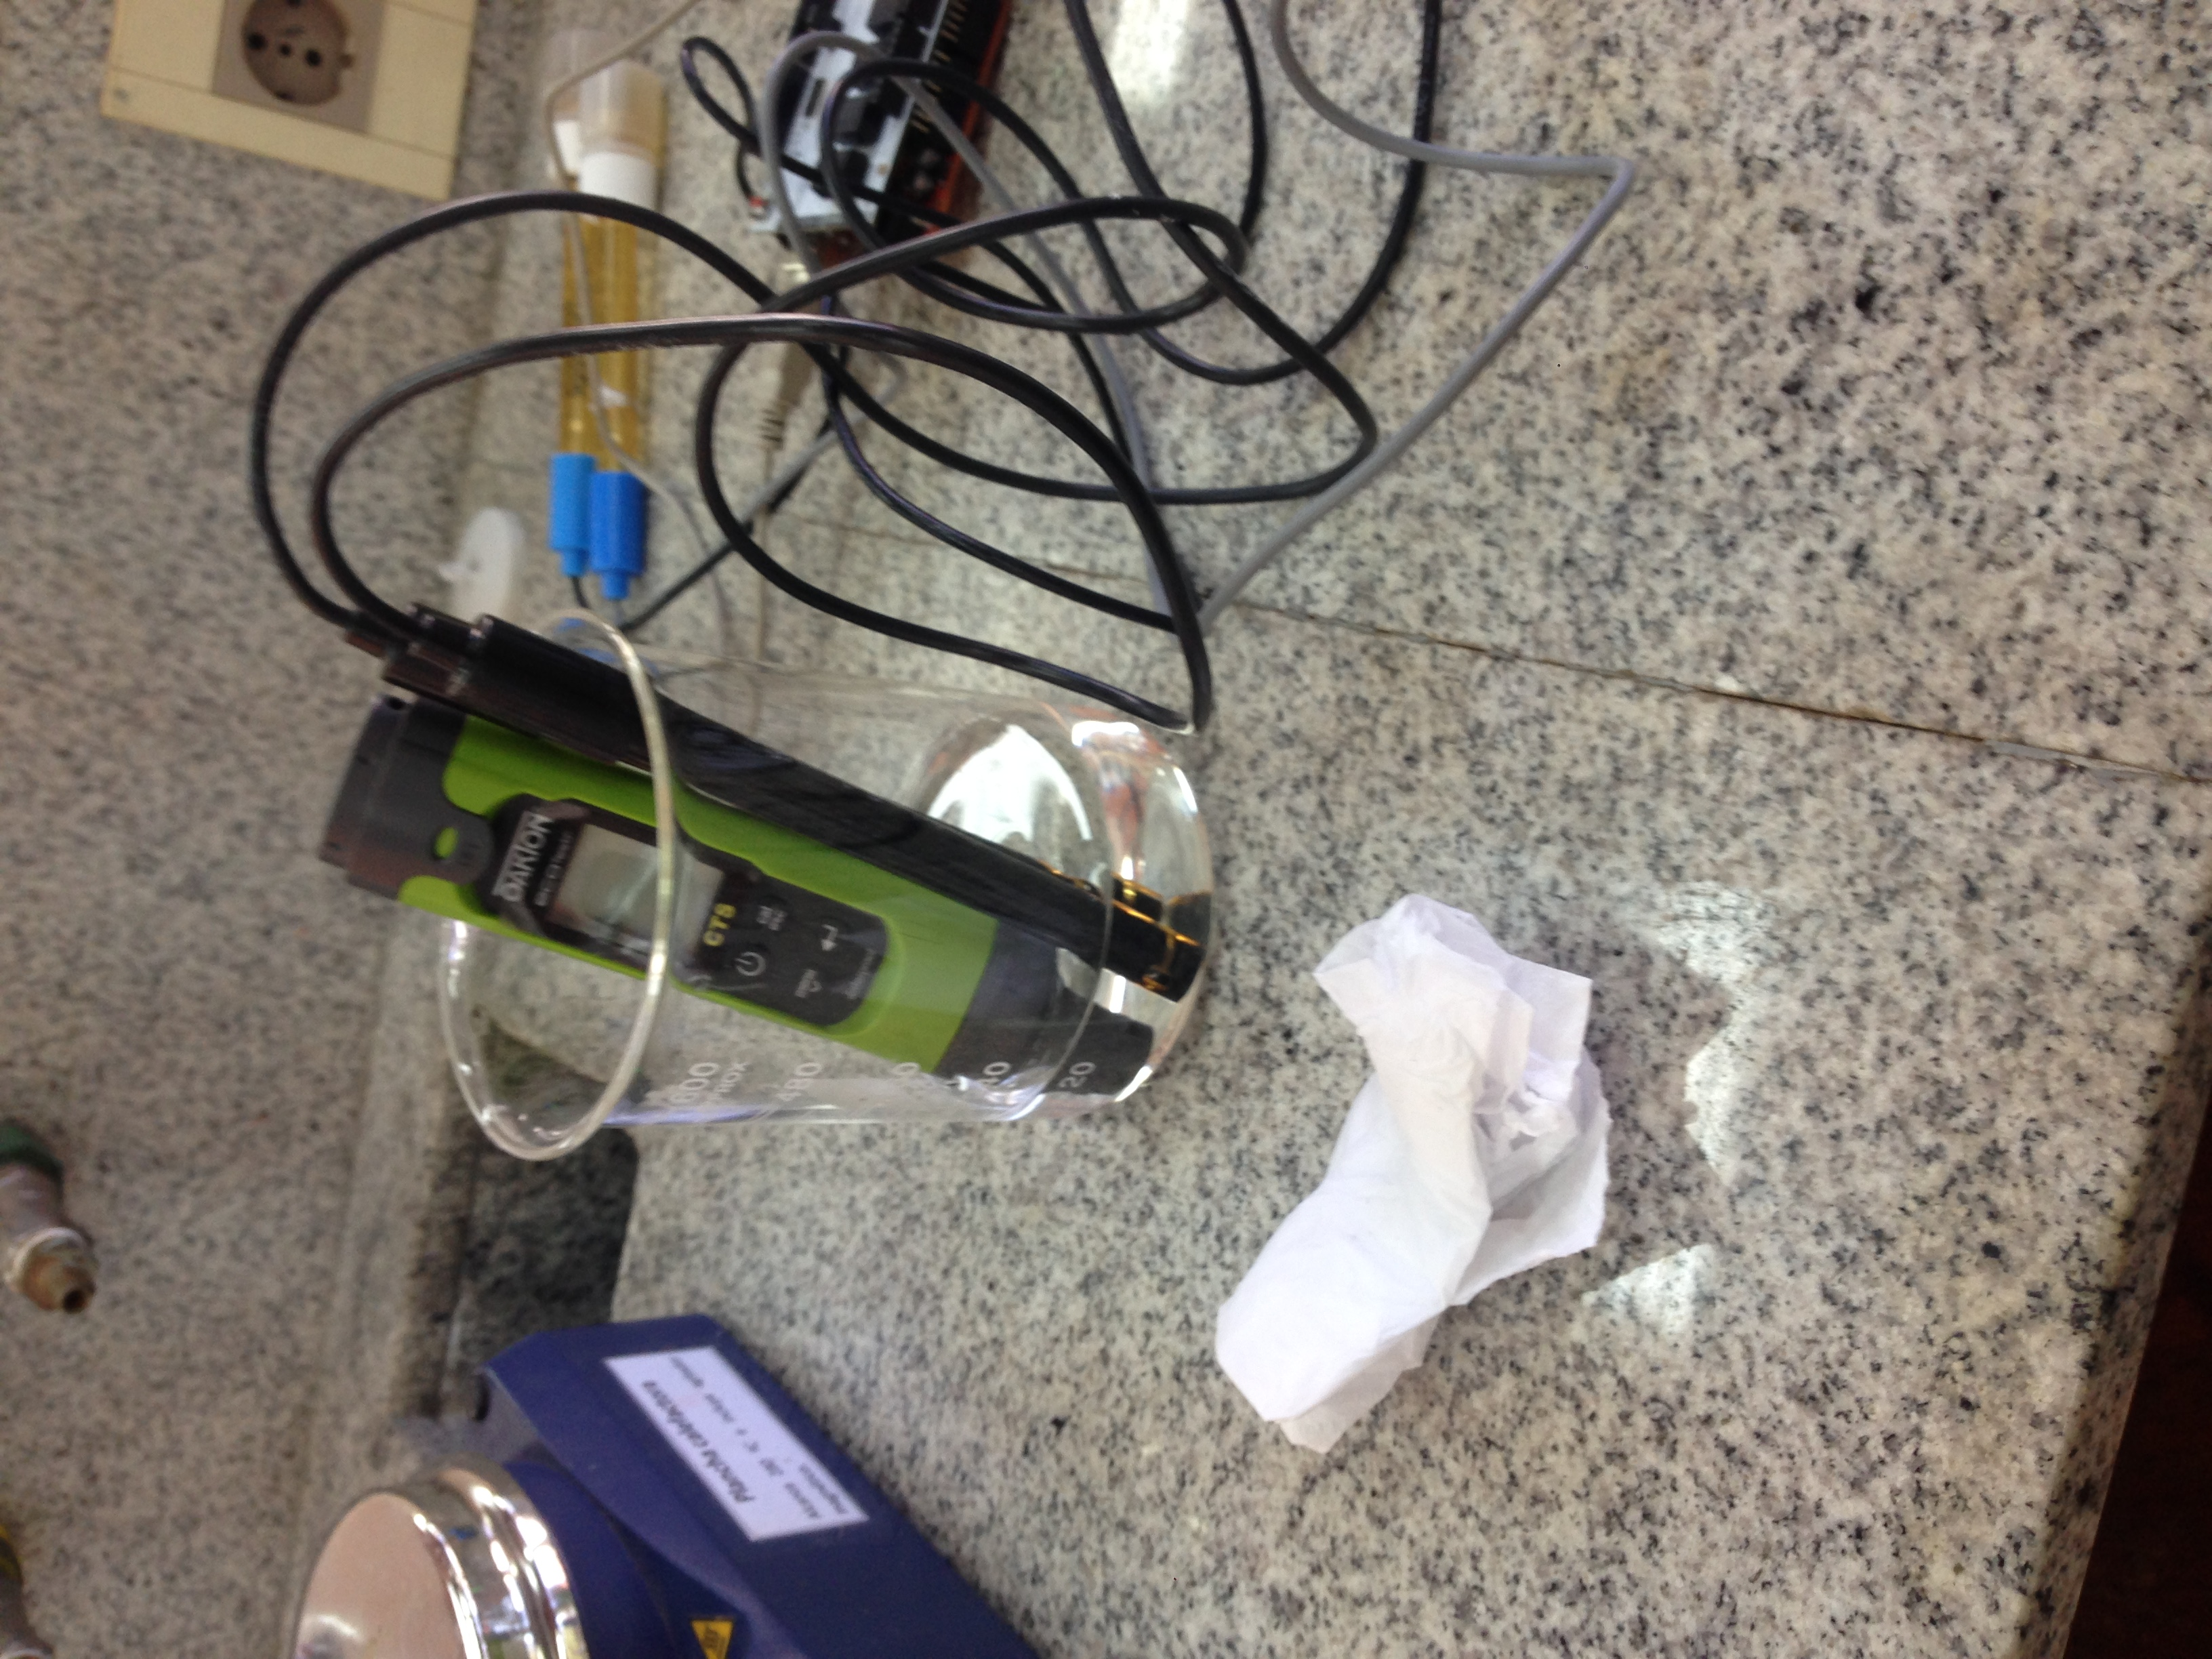
\includegraphics[angle=270,width=\textwidth]{Imagenes/cap4/qca3.jpg}
         \caption{Muestreo de CE}
         \label{fig: Muestreo de CE}
     \end{subfigure}
        \caption{Muestreo en el laboratorio qu\'imica - FIUNA}
        \label{fig:muestreoQCA}
\end{figure}


\newpage
\subsubsection{Muestra 1. Sensor de temperatura}
    \begin{table}[H]
        \protect\caption[Muestra 1: Destilada ]{Muestra 1: Agua de destilada.}
        \label{tab:TMuestra1}
        \centering
        \begin{tabular}{c c c}
            \hline
            \multicolumn{3}{c}{\textbf{Muestra 1: Agua de destilada}} \\
             \hline
            \multicolumn{3}{c}{\textbf{Recipiente 1}} \\
            \hline
            \textbf{Lectura}&\textbf{LSD ($^{\circ}$C)}&\textbf{Qca ($^{\circ}$C)} \\
            \hline
            {1}& $25.7$&$25.5$ \\ 
            % \hline
            {2}& $25.4$&$25.5$ \\ 
            % \hline
             {3}& $25.6$&$25.6$\\  
            % \hline
            {4}& $25.4$&$25.5$\\ 
            % \hline
            {5}& $25.2$&$25.6$ \\
            \hline
                       \multicolumn{3}{c}{\textbf{Recipiente 2}} \\
            \hline
            \textbf{Lectura}&\textbf{LSD ($^{\circ}$C)}&\textbf{Qca ($^{\circ}$C)} \\
            \hline
            {1}& $25.5$&$25.3$ \\ 
            % \hline
            {2}& $25.4$&$25.3$ \\ 
            % \hline
             {3}& $25.2$&$25.3$\\  
            % \hline
            {4}& $24.8$&$25.4$\\ 
            % \hline
            {5}& $24.6$&$25.4$ \\ 
            \hline
            \multicolumn{3}{c}{\textbf{Recipiente 3}} \\
            \hline
            \textbf{Lectura}&\textbf{LSD ($^{\circ}$C)}&\textbf{Qca´($^{\circ}$C)} \\
            \hline
            {1}& $24.6$&$25.4$ \\ 
            % \hline
            {2}& $25.6$&$25.6$ \\ 
            % \hline
             {3}& $25.9$&$25.6$\\  
            % \hline
            {4}& $25.6$&$25.4$\\ 
            % \hline
            {5}& $25.4$&$25.3$ \\ 
            \hline
        \end{tabular}
        \vspace{5mm}
        \newline
        \hfill \textbf{Fuente: }Elaboración Propia.
    \end{table}

% Grafico M1T
\begin{figure}[H]
        \centering
        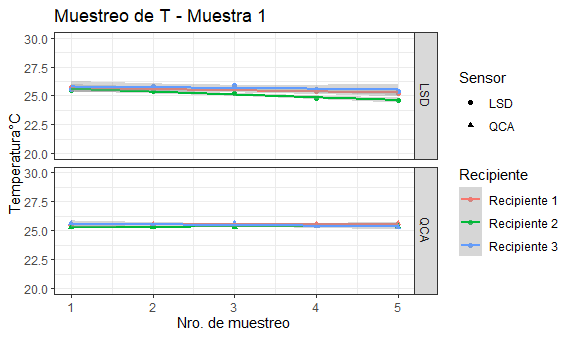
\includegraphics[width=0.75\linewidth]{Imagenes/cap4/T_M1.png}
        \caption {Muestreo de temperatura. }{\textbf{Fuente:}
        Elaboraci\'on Propia. }
        \label{fig:M1T}
    \end{figure}
    
\subsubsection{Muestra 1. Sensor Conductividad El\'ectrica}
    \begin{table}[H]
        \protect\caption[Muestra 1: Destilada ]{Muestra 1: Agua de destilada.}
        \label{tab:TMuestra1}
        \centering
        \begin{tabular}{c c c}
            \hline
            \multicolumn{3}{c}{\textbf{Muestra 1: Agua de destilada}} \\
             \hline
            \multicolumn{3}{c}{\textbf{Recipiente 1}} \\
            \hline
            \textbf{Lectura}&\textbf{LSD ($\mu S/cm$)}&\textbf{Qca ($\mu S/cm$)} \\
            \hline
            {1}& $0$&$0$ \\ 
            % \hline
            {2}& $0$&$0$ \\ 
            % \hline
             {3}& $0$&$0$\\  
            % \hline
            {4}& $0$&$0$\\ 
            % \hline
            {5}& $0$&$0$ \\
            \hline
                       \multicolumn{3}{c}{\textbf{Recipiente 2}} \\
            \hline
            \textbf{Lectura}&\textbf{LSD ($\mu S/cm$)}&\textbf{Qca ($\mu S/cm$)} \\
            \hline
            {1}& $0$&$0$ \\ 
            % \hline
            {2}& $0$&$0$ \\ 
            % \hline
            {3}& $0$&$0$\\  
            % \hline
            {4}& $0$&$0$\\ 
            % \hline
            {5}& $0$&$0$ \\
            \hline
            \multicolumn{3}{c}{\textbf{Recipiente 3}} \\
            \hline
            \textbf{Lectura}&\textbf{LSD ($\mu S/cm$)}&\textbf{Qca ($\mu S/cm$)} \\
            \hline
            {1}& $0$&$0$ \\ 
            % \hline
            {2}& $0$&$0$ \\ 
            % \hline
             {3}& $0$&$0$\\  
            % \hline
            {4}& $0$&$0$\\ 
            % \hline
            {5}& $0$&$0$ \\
            \hline
        \end{tabular}
        \vspace{5mm}
        \newline
        \hfill \textbf{Fuente: }Elaboración Propia.
    \end{table}

% Grafico M1CE
    \begin{figure}[H]
        \centering
        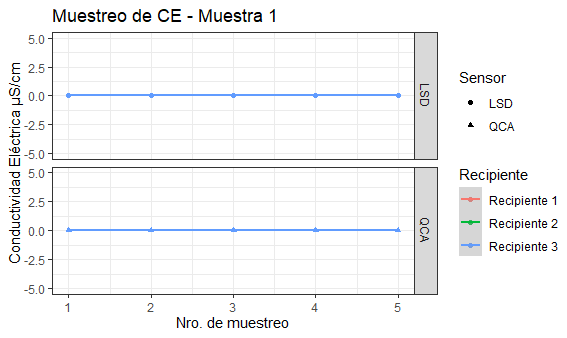
\includegraphics[width=0.75\linewidth]{Imagenes/cap4/CE_M1.png}
        \caption {Muestreo de conductividad el\'ectrica. }{\textbf{Fuente:}
        Elaboraci\'on Propia. }
        \label{fig:M1CE}
    \end{figure}

\subsubsection{Muestra 1. Sensor de pH}
    \begin{table}[H]
        \protect\caption[Muestra 1: Destilada ]{Muestra 1: Agua de destilada.}
        \label{tab:TMuestra1}
        \centering
        \begin{tabular}{c c c}
            \hline
            \multicolumn{3}{c}{\textbf{Muestra 1: Agua de destilada}} \\
             \hline
            \multicolumn{3}{c}{\textbf{Recipiente 1}} \\
            \hline
            \textbf{Lectura}&\textbf{LSD ($pH$)}&\textbf{Qca ($pH$)} \\
            \hline
            {1}& $6.898$&$8.27$ \\ 
            % \hline
            {2}& $6.853$&$7.86$ \\ 
            % \hline
            {3}& $6.856$&$7.36$\\  
            % \hline
            {4}& $6.809$&$6.82$\\ 
            % \hline
            {5}& $6.715$&$6.86$ \\
            \hline
            \multicolumn{3}{c}{\textbf{Recipiente 2}} \\
            \hline
            \textbf{Lectura}&\textbf{LSD ($pH$)}&\textbf{Qca ($pH$)} \\
            \hline
            {1}& $6.555$&$6.59$ \\ 
            % \hline
            {2}& $6.303$&$6.88$ \\ 
            % \hline
            {3}& $5.919$&$6.76$\\  
            % \hline
            {4}& $5.502$&$6.65$\\ 
            % \hline
            {5}& $5.171$&$6.62$ \\
            \hline
            \multicolumn{3}{c}{\textbf{Recipiente 3}} \\
            \hline
            \textbf{Lectura}&\textbf{LSD ($pH$)}&\textbf{Qca ($pH$)} \\
            \hline
            {1}& $6.495$&$6.86$ \\ 
            % \hline
            {2}& $6.440$&$6.77$ \\ 
            % \hline
             {3}& $6.316$&$6.49$\\  
            % \hline
            {4}& $6.711$&$6.18$\\ 
            % \hline
            {5}& $6.613$&$6.37$ \\
            \hline
        \end{tabular}
        \vspace{5mm}
        \newline
        \hfill \textbf{Fuente: }Elaboración Propia.
    \end{table}

% Grafico M1Ph
    \begin{figure}[H]
        \centering
        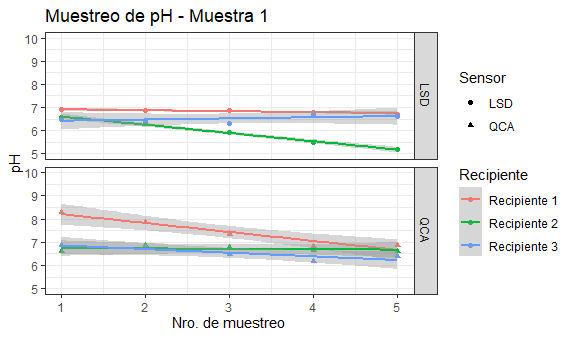
\includegraphics[width=0.75\linewidth]{Imagenes/cap4/pH_M1.png}
        \caption {Muestreo de pH. }{\textbf{Fuente:}
        Elaboraci\'on Propia. }
        \label{fig:M1PH}
    \end{figure}

\subsubsection{An\'alisis de Datos. Muestra 1}
% Please add the following required packages to your document preamble:

\begin{table}[H]
\protect\caption[Muestra 1: Destilada ]{Estad\'isticas de mediciones: Muestra 1.}
\label{tab:AnalisisM1}
\begin{tabular}{l ccc|ccc}
\hline
\textbf{Muestra 1  }& \multicolumn{3}{c}{LSD} & \multicolumn{3}{c}{QCA}  \\ 
\begin{tabular}[c]{@{}l@{}}An\'alisis de datos\end{tabular} & \multicolumn{1}{c}{\begin{tabular}[c]{@{}c@{}}T \\$ ^{\circ}C$\end{tabular}} & \multicolumn{1}{c}{pH}        & \begin{tabular}[c]{@{}c@{}}CE\\ $\mu S/cm$\end{tabular} & \multicolumn{1}{c}{\begin{tabular}[c]{@{}c@{}}T \\$ ^{\circ}C$\end{tabular}} & \multicolumn{1}{c}{pH}        & \multicolumn{1}{c}{\begin{tabular}[c]{@{}c@{}}CE\\ $\mu S/cm$\end{tabular}} \\ 
\hline
Desviaci\'on Est\'andar & \multicolumn{1}{c}{0.349} & \multicolumn{1}{c}{0.511} & 0                                                  & \multicolumn{1}{c}{0.118}                                       & \multicolumn{1}{c}{0.551} & \multicolumn{1}{c}{0}                                                  \\ 
Varianza                                                                        & \multicolumn{1}{c}{0.122}                                       & \multicolumn{1}{c}{0.261} & 0                                                  & \multicolumn{1}{c}{0.014}                                      & \multicolumn{1}{c}{0.304} & \multicolumn{1}{c}{0}                                                  \\ 
Error Estándar                                                                  & \multicolumn{1}{c}{0.090}                                      & \multicolumn{1}{c}{0.132} & 0                                                  & \multicolumn{1}{c}{0.0306}                                      & \multicolumn{1}{c}{0.142} & \multicolumn{1}{c}{0}                                                  \\ 
Mínimo  &   \multicolumn{1}{c}{24.60}  & \multicolumn{1}{r}{5.171} & 0 & \multicolumn{1}{c}{25.30} & \multicolumn{1}{r}{6.180} & 0 \\
% \hline
Máximo  & \multicolumn{1}{c}{25.90}    & \multicolumn{1}{c}{6.898} & 0 & \multicolumn{1}{c}{25.60}  & \multicolumn{1}{c}{8.270} & 0  \\ 
% \hline
Promedio & \multicolumn{1}{c}{25.41}   & \multicolumn{1}{c}{6.410} & 0 & \multicolumn{1}{c}{25.45} & \multicolumn{1}{c}{6.889} & 0 
\\ 
\hline
\end{tabular}
\vspace{5mm}
\newline
\hfill \textbf{Fuente: }Elaboración Propia.
\end{table}

En la tabla \ref{tab:AnalisisM1}, se puede observar algunos par\'metros estad\'isticos calculados, a partir de los registros recolectados en el muestreo de los recipientes de la muestra 1, el cual arrojo los siguientes resultados. La desviaci\'on est\'andar en el caso de la temperatura, presenta en ambos caso un \'indice bajo m\'as aun para el equipo de QCA, por lo cual indica que la mayor parte de los datos de una muestra tienden a estar agrupados cerca de su media. En caso del pH la desviaci\'on est\'andar es un poco mayor, pero de igual manera baja, por lo tanto, tambi\'en tienen tendencia que las lecturas se agrupen cerca de la media. La varianza sigue la misma tendencia de la desviaci\'on est\'andar, por lo tanto, todos los datos recolectados no presentan dispersi\'on. El error est\'andar, presenta valores bajos en todo los par\'ametros, el cual sugiere que los valores recolectados son uniforme y se encuentran cerca de la media. Los valores mínimos recolectados en el caso de la temperatura presentan una deferencia de 0,7 $ ^{\circ}C$ siendo 25.3 $ ^{\circ}C$ la menor lectura registrada por el sensor de QCA, en el caso del pH la diferencia entre los mínimos fue de 1.009 pH, siendo 5.171 pH la menor lectura registrada por el sensor de LSD. Los valores m\'aximo recolectados en el caso de la temperatura presentan una deferencia de 0,3 $ ^{\circ}C$ siendo 25.90 $ ^{\circ}C$ la mayor lectura registrada por el sensor de LSD, en el caso del pH la diferencia entre los m\'aximos fue de 1.372 pH, siendo 8.270 pH la mayor lectura registrada por el sensor de QCA. El promedio de las mediciones fueron cercanas con una diferencia de 7$\%$ en el caso del pH, siendo el promedio de los datos de pH registrado por el sensor de QCA 6.889 pH contra el promedio de pH registrado por el sensor LSD igual a 6.41 pH, en el caso de los resultados promedios registrados de la temperatura la diferencia entre los resultados fue menor al 0.5$\%$ siendo la temperatura promedio del sensor LSD igual a 24.41$ ^{\circ}C$ y la temperatura promedio del sensor de QCA igual a 25.25$^{\circ}C$. En este an\'alisis de datos correspondiente a la muestra 1, no sé describi\'o los datos recolectados por el sensor de CE, ya que en ambos sensores se obtuvieron los mismos resultados iguales a 0 $\mu S/cm$, tal como se espera para este tipo de muestra.

\begin{table}[]
\caption{Relaci\'on entre los equipos de sensores}
\label{tab:VaCoM1}
\centering
\begin{tabular}{llll} 
\toprule
& T   &  pH    & CE \\
\midrule
Covarianza  & 0.0125& 0.111 & 0                \\
Correlación & 0.301& 0.395 & 0        \\
\bottomrule
\end{tabular}
\\ \textbf{Fuente: }Elaboración Propia.
\end{table}     
% https://sitiobigdata.com/2019/10/26/covarianza-y-correlacion/


En la tabla \ref{tab:VaCoM1}, se analizan los resultados de covarianza y correlación de las muestras, en el caso de la temperatura y pH se obtuvieron unas covarianzas positivas el cual indica que ambas lecturas varían en la misma dirección, as\'i mismo en ambos par\'ametros se obtuvieron correlaciones positivas lo cual indica que son directamente proporcionales entre sí, la media varía en la misma dirección con el factor del valor del coeficiente de correlación. Luego de analizar los resultados obtenidos en el caso de la muestra 1, se puede concluir que ambos sensores presentan lecturas cercanas, con baja dispersi\'on. 

%% Muestra nro 2: Agua de Pozo
\subsubsection{Muestra 2.Temperatura}
    \begin{table}[H]
        \protect\caption[Muestra 2: Agua de pozo ]{Muestra 2: Agua de pozo.}
        \label{tab:TMuestra2}
        \centering
        \begin{tabular}{c c c}
            \hline
            \multicolumn{3}{c}{\textbf{Muestra 2: Agua de pozo.}} \\
             \hline
            \multicolumn{3}{c}{\textbf{Recipiente 1}} \\
            \hline
            \textbf{Lectura}&\textbf{LSD($^{\circ}$C)}&\textbf{Qca($^{\circ}$C)} \\
            \hline
            {1}& $23.6$&$25.1$ \\ 
            % \hline
            {2}& $22.9$&$24.9$ \\ 
            % \hline
             {3}& $22.6$&$24.8$\\  
            % \hline
            {4}& $22.5$&$24.6$\\ 
            % \hline
            {5}& $22.3$&$24.6$ \\
            \hline
                       \multicolumn{3}{c}{\textbf{Recipiente 2}} \\
            \hline
            \textbf{Lectura}&\textbf{LSD($^{\circ}$C)}&\textbf{Qca($^{\circ}$C)} \\
            \hline
            {1}& $24.4$&$24.4$ \\ 
            % \hline
            {2}& $24.0$&$24.2$ \\ 
            % \hline
             {3}& $23.9$&$24.0$\\  
            % \hline
            {4}& $23.9$&$23.9$\\ 
            % \hline
            {5}& $23.8$&$23.9$ \\ 
            \hline
            \multicolumn{3}{c}{\textbf{Recipiente 3}} \\
            \hline
            \textbf{Lectura}&\textbf{LSD($^{\circ}$C)}&\textbf{Qca($^{\circ}$C)} \\
            \hline
            {1}& $22.2$&$23.9$ \\ 
            % \hline
            {2}& $21.9$&$24.0$ \\ 
            % \hline
             {3}& $21.5$&$23.8$\\  
            % \hline
            {4}& $21.4$&$23.7$\\ 
            % \hline
            {5}& $21.2$&$23.6$ \\ 
            \hline
        \end{tabular}
        \vspace{5mm}
        \newline
        \hfill \textbf{Fuente: }Elaboración Propia.
    \end{table}

% Gráfico M2T
    \begin{figure}[H]
        \centering
        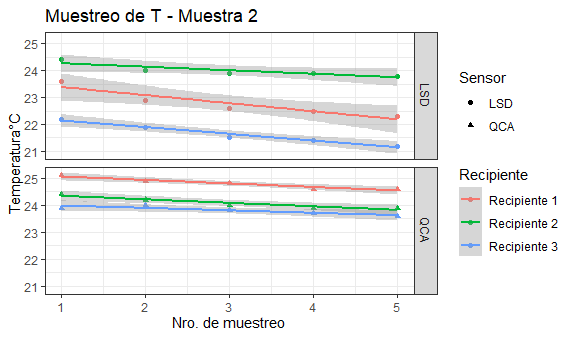
\includegraphics[width=0.75\linewidth]{Imagenes/cap4/T_M2.png}
        \caption {Muestreo de temperatura. }{\textbf{Fuente:}
        Elaboraci\'on Propia. }
        \label{fig:M2T}
    \end{figure}

\subsubsection{Muestra 2. Sensor Conductividad El\'ectrica }
    \begin{table}[H]
        \protect\caption[Muestra 2: Agua de pozo ]{Muestra 2: Agua de pozo.}
        \label{tab:CEMuestra2}
        \centering
        \begin{tabular}{c c c }
            \hline
            \multicolumn{3}{c}{\textbf{Muestra 2: Agua de pozo}} \\
             \hline
            \multicolumn{3}{c}{\textbf{Recipiente 1}} \\
            \hline
            \textbf{Lectura}&\textbf{LSD ($\mu S/cm$)}&\textbf{Qca ($\mu S/cm$)} \\
            \hline
            {1}& $81.39$&$100$ \\ 
            {2}& $80.12$&$90$ \\ 
            {3}&$80.05$&$90$\\  
            {4}& $80.55$&$100$\\ 
            {5}& $80.10$&$90$ \\
            \hline
                       \multicolumn{3}{c}{\textbf{Recipiente 2}} \\
            \hline
            \textbf{Lectura}&\textbf{LSD ($\mu S/cm$)}&\textbf{Qca ($\mu S/cm$)} \\
            \hline
            {1}& $80.32$&$80$ \\ 
            {2}& $80.36$&$80$ \\ 
            {3}&$80.40$&$80$  \\  
            {4}& $80.45$&$80$ \\ 
            {5}& $80.49$&$80$ \\ 
            \hline
            \multicolumn{3}{c}{\textbf{Recipiente 3}} \\
            \hline
            \textbf{Lectura}&\textbf{LSD ($\mu S/cm$)}&\textbf{Qca($\mu S/cm$)} \\
            \hline
            {1}& $119.60$&$130$ \\ 
            {2}& $110.30$&$130$ \\ 
            {3}&$118.90$&$130$  \\  
            {4}& $117.10$&$130$ \\ 
            {5}& $118.40$&$130$ \\ 
            \hline
        \end{tabular}
        \vspace{5mm}
        \newline
        \hfill \textbf{Fuente: }Elaboración Propia.
    \end{table}

% Gráfico M2CE
    \begin{figure}[H]
        \centering
        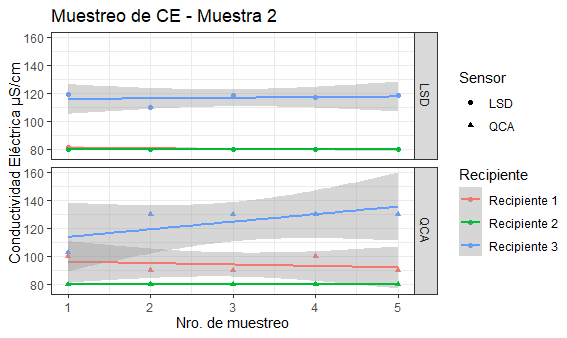
\includegraphics[width=0.75\linewidth]{Imagenes/cap4/CE_M2.png}
        \caption {Muestreo de conductividad el\'ectrica. }{\textbf{Fuente:}
        Elaboraci\'on Propia. }
        \label{fig:M2CE}
    \end{figure}

\subsubsection{Muestra 2. Sensor de pH}
    \begin{table}[H]
        \protect\caption[Muestra 2: Agua de pozo ]{Muestra 2: Agua de pozo.}
        \label{tab:phMuestra2}
        \centering
        \begin{tabular}{c c c}
            \hline
            \multicolumn{3}{c}{\textbf{Muestra 2: Agua de pozo.}} \\
             \hline
            \multicolumn{3}{c}{\textbf{Recipiente 1}} \\
            \hline
            \textbf{Lectura}&\textbf{LSD ($pH$)}&\textbf{Qca ($pH$)} \\
            \hline
            {1}& $5.569$&$6.12$ \\ 
            {2}& $5.513$&$6.15$ \\ 
            {3}& $5.458$&$6.13$\\  
            {4}& $5.402$&$6.17$\\ 
            {5}& $5.498$&$6.20$ \\
            \hline
            \multicolumn{3}{c}{\textbf{Recipiente 2}} \\
            \hline
            \textbf{Lectura}&\textbf{LSD ($pH$)}&\textbf{Qca ($pH$)} \\
            \hline
            {1}& $5.157$&$5.94$ \\ 
            {2}& $5.251$&$5.96$ \\ 
            {3}& $5.552$&$5.98$ \\  
            {4}& $5.595$&$6.03$ \\ 
            {5}& $5.551$&$6.01$ \\
            \hline
            \multicolumn{3}{c}{\textbf{Recipiente 3}} \\
            \hline
            \textbf{Lectura}&\textbf{LSD ($pH$)}&\textbf{Qca ($pH$)} \\
            \hline
            {1}& $5.582$&$5.91$ \\ 
            {2}& $5.624$&$6.04$ \\ 
            {3}&$5.732$&$6.11$ \\  
            {4}& $5.918$&$6.09$\\ 
            {5}& $5.936$&$6.18$ \\
            \hline
        \end{tabular}
        \vspace{5mm}
        \newline
        \hfill \textbf{Fuente: }Elaboración Propia.
    \end{table}

% Gráfico M2pH
    \begin{figure}[H]
        \centering
        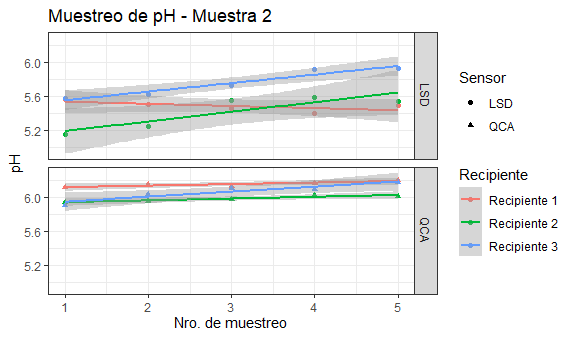
\includegraphics[width=0.75\linewidth]{Imagenes/cap4/pH_M2.png}
        \caption {Muestreo de pH. }{\textbf{Fuente:}
        Elaboraci\'on Propia. }
        \label{fig:M2PH}
    \end{figure}

\subsection{An\'alsis de Datos. Muestra 2}

\begin{table}[H]
    \protect\caption[Muestra 2: Agua de pozo ]{Resumen de mediciones: Muestra 2.}
\label{tab:AnalisisM2}

    \begin{tabular}{lccc|ccc}
    \hline
    Muestra 2 & 
    \multicolumn{3}{c}{LSD} & 
    \multicolumn{3}{c}{QCA}  \\
    \textbf{\begin{tabular}[c]{@{}l@{}}An\'alisis de datos
    \end{tabular}} & \multicolumn{1}{c}{\begin{tabular}[c]{@{}c@{}}T \\ $^{\circ} C$ 
    \end{tabular}} & \multicolumn{1}{c}{pH}        & 
    \begin{tabular}[c]{@{}c@{}}CE\\ $\mu S/cm$\end{tabular} & \multicolumn{1}{c}{\begin{tabular}[c]{@{}c@{}}T \\ $^{\circ} C$
    \end{tabular}} & 
    \multicolumn{1}{c}{pH}        & 
    \multicolumn{1}{c}{\begin{tabular}[c]{@{}c@{}}CE\\ $\mu S/cm$\end{tabular}} \\ 
    \hline
    M\'inimo & 
    \multicolumn{1}{c}{21.20} & 
    \multicolumn{1}{c}{5.157} & 80.05   & \multicolumn{1}{c}{23.60}& 
    \multicolumn{1}{c}{5.910} & 80.0  \\ 
    M\'aximo & 
    \multicolumn{1}{c}{24.40} & 
    \multicolumn{1}{c}{5.936} & 119.60 & 
    \multicolumn{1}{c}{25.10} & 
    \multicolumn{1}{c}{6.200} & 130.0  \\ Promedio & \multicolumn{1}{c}{22.81} & 
    \multicolumn{1}{c}{5.556} & 92.57  & \multicolumn{1}{c}{24.23} & 
    \multicolumn{1}{c}{6.068} & 101.3  \\ 
    Desviaci\'on Est\'andar  & 
    \multicolumn{1}{c}{1.063}  & 
    \multicolumn{1}{c}{0.2077} & {17.89} & \multicolumn{1}{c}{0.472} &
    \multicolumn{1}{c}{0.0934} & 
    \multicolumn{1}{c}{21.995} \\ 
    Varianza & 
    \multicolumn{1}{c}{1.130} &
    \multicolumn{1}{c}{0.0431} & 320.28  & \multicolumn{1}{c}{0.223} & 
    \multicolumn{1}{c}{0.00873} & 
    \multicolumn{1}{c}{483.8}                              \\
    Error Est\'andar & 
    \multicolumn{1}{c}{0.274}  & 
    \multicolumn{1}{c}{0.0536} & {4.62} & 
    \multicolumn{1}{c}{0.122} & 
    \multicolumn{1}{c}{0.024} & 
    \multicolumn{1}{c}{5.68}         \\ \hline
    \end{tabular}
\end{table}

En la tabla \ref{tab:AnalisisM2}, se puede observar algunos par\'ametros estad\'isticos calculados, a partir de los registros recolectados en el muestreo de los recipientes de la muestra 2, el cual arrojo los siguientes resultados. 
La desviaci\'on est\'andar m\'as elevada se registr\'o en el par\'ametro de conductividad el/éctrica, siendo el mayor el registrado por el sensor de qu/ímica igual a 21.9 un  4\%  mayor a la desviación del LSD, en los resultados de  los otros par\'ametros, se registra un desviaci\'on menor en sensores de QCA,   . 
La varianza sigue la misma tendencia de la desviaci\'on est\'andar, la conductividad el\'ectrica presenta una mayor dispersi\'on. 
El error est\'andar, presenta valores bajos en los par\'ametros de pH y QCA, el cual sugiere que los valores recolectados son uniforme y se encuentran cerca de la media. 
Los valores mínimos recolectados en el caso de la temperatura presentan una deferencia de 2,4 $ ^{\circ}C$ siendo 21.2$ ^{\circ}C$ la menor lectura registrada por el sensor de LSD, en el caso del pH la diferencia entre los mínimos fue de 0.753 pH, siendo 5.157 pH la menor lectura registrada por el sensor de LSD, la m\'inima conductividad el\'ectrica registrado fue de 80.00$\mu S/cm$ con una variaci\'on muy baja entre los sensores. 
Los valores m\'aximo recolectados en el caso de la temperatura presentan una deferencia de 0,7 $ ^{\circ}C$ siendo 25.1 $ ^{\circ}C$ la mayor lectura registrada por el sensor de QCA, en el caso del pH la diferencia entre los m\'aximos fue de 0.264 pH, siendo 6.20 pH la mayor lectura registrada por el sensor de QCA, la conductividad el\'ectrica m\'as alta registrada fue de 130.00 $\mu S/cm$ con con una diferencia de 10.4 $\mu S/cm$ con respecto a la mayor lectura registrada en el sensor QCA.
El promedio de las mediciones fueron cercanas con una diferencia de 9.16$\%$ en el caso del pH, siendo el promedio de los datos de pH registrado por el sensor de QCA 5.556 pH contra el promedio de pH registrado por el sensor LSD igual a 6.068 pH, en el caso de los resultados promedios registrados de la temperatura la diferencia entre los resultados fue menor al 9.41$\%$ siendo la temperatura promedio del sensor LSD igual a 22.81$ ^{\circ}C$ y la temperatura promedio del sensor de QCA igual a 24.23$^{\circ}C$, los promedio de las mediciones de los sensores de conductividad eléctrica entre los sensores tienen diferencia de 9.14$\%$, siendo el promedio de los datos de CE registrado por el sensor de QCA 101.3 contra el promedio de CE registrado por el sensor LSD igual a 92.57$\mu S/cm$ .
En este an\'alisis de datos correspondiente a la muestra 2, se observan los mismos patrones, los resultados finales con valores cercanos, con un margen de diferencia menor al 10\% entre ambos sensores. 


\begin{table}[H]
\caption{Relaci\'on entre los equipos de sensores}
\label{tab:VaCoM2}
\centering
\begin{tabular}{llll} 
\toprule
& T   &  pH    & CE \\
\midrule
Covarianza  &0.168 & 0.00734 & 373.89        \\
Correlaci\'on & 0.334& 0.3782 & 0.949        \\
\bottomrule
\end{tabular}
\\ \textbf{Fuente: }Elaboración Propia.
\end{table} 
En un analis de la tabla \ref{tab:VaCoM2}, donde se encuentran los resultados de covarianza y correlación de las muestras, en el caso de la temperatura, conductividad el\'ectrica y pH se obtuvieron unos valores de covarianzas positivas el cual indica que ambas lecturas varían en la misma dirección, as\'i mismo en los tres par\'ametros se obtuvieron correlaciones positivas menores a 1, refleja que se da una correlación positiva entre sí, la media varía en la misma dirección con el factor del valor del coeficiente de correlación. Luego de analizar los resultados obtenidos en el caso de la muestra 2, se puede concluir que ambos sensores presentan lecturas cercanas,relacionadas entre s\'i, con baja dispersi\'on. 

\subsubsection{Muestra 3. Sensor de Temperatura}
  \begin{table}[H]
        \protect\caption[Muestra 3: Agua de laguna]{Muestra 3: Agua de laguna.}
        \label{tab:TMuestra3}
        \centering
        \begin{tabular}{c c c}
            \hline
            \multicolumn{3}{c}{\textbf{Muestra 3: Agua de laguna.}} \\
             \hline
            \multicolumn{3}{c}{\textbf{Recipiente 1}} \\
            \hline
            \textbf{Lectura}&\textbf{LSD ($^{\circ} C$)}&\textbf{Qca ($^{\circ} C$)} \\
            \hline
            {1}& $22.3$&$22.1$ \\ 
            {2}& $22.2$&$22.3$ \\ 
            {3}& $22.3$&$22.1$ \\  
            {4}& $22.1$&$21.9$ \\ 
            {5}& $22.1$&$21.8$ \\
            \hline
            \multicolumn{3}{c}{\textbf{Recipiente 2}} \\
            \hline
            \textbf{Lectura}&\textbf{LSD ($^{\circ} C$)}&\textbf{Qca ($^{\circ} C$)} \\
            \hline
            {1}& $22.7$&$21.8$ \\ 
            {2}& $22.7$&$22.9$ \\ 
            {3}& $22.7$&$22.9$ \\  
            {4}& $22.7$&$22.7$ \\ 
            {5}& $22.7$&$22.7$ \\
            \hline
            \multicolumn{3}{c}{\textbf{Recipiente 3}} \\
            \hline
            \textbf{Lectura}&\textbf{LSD ($^{\circ} C$)}&\textbf{Qca ($^{\circ} C$)} \\
            \hline
            {1}& $22.7$&$22.2$\\ 
            {2}& $22.8$&$22.2$\\ 
            {3}&$22.8$&$22.2$ \\  
            {4}& $22.9$&$22.3$\\ 
            {5}& $22.9$&$22.4$\\
            \hline
        \end{tabular}
        \vspace{5mm}
        \newline
        \hfill \textbf{Fuente: }Elaboración Propia.
    \end{table}




% Gráfico M3T
    \begin{figure}[H]
        \centering
        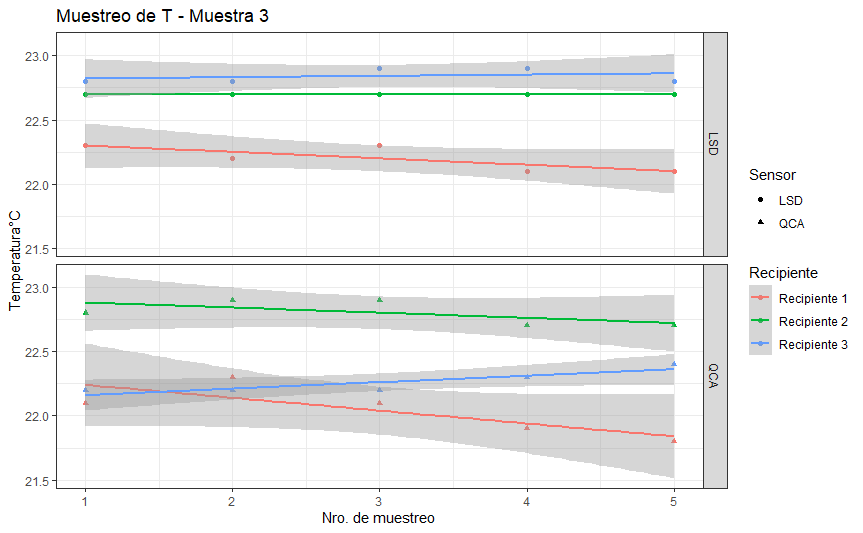
\includegraphics[width=0.75\linewidth]{Imagenes/cap4/T_M3.png}
        \caption {Muestreo de pH. }{\textbf{Fuente:}
        Elaboraci\'on Propia. }
        \label{fig:M3T}
    \end{figure}

\subsubsection{Muestra 3. Sensor Conductividad El\'ectrica}
  \begin{table}[H]
        \protect\caption[Muestra 3: Agua de laguna]{Muestra 3: Agua de laguna.}
        \label{tab:CEMuestra3}
        \centering
        \begin{tabular}{c c c}
            \hline
            \multicolumn{3}{c}{\textbf{Muestra 3: Agua de laguna.}} \\
             \hline
            \multicolumn{3}{c}{\textbf{Recipiente 1}} \\
            \hline
            \textbf{Lectura}&\textbf{LSD ($\mu S/cm$)}&\textbf{Qca ($\mu S/cm$)} \\
            \hline
            {1}& $36.35$&$50$ \\ 
            {2}& $35.18$&$52$ \\ 
            {3}& $35.15$&$50$ \\  
            {4}& $34.87$&$50$ \\ 
            {5}& $33.70$&$51$ \\
            \hline
            \multicolumn{3}{c}{\textbf{Recipiente 2}} \\
            \hline
            \textbf{Lectura}&\textbf{LSD ($\mu S/cm$)}&\textbf{Qca ($\mu S/cm$)} \\
            \hline
            {1}& $32.24$&$52$ \\ 
            {2}& $34.01$&$51$ \\ 
            {3}& $34.13$&$50$ \\  
            {4}& $33.03$&$53$ \\ 
            {5}& $32.75$&$52$ \\
            \hline
            \multicolumn{3}{c}{\textbf{Recipiente 3}} \\
            \hline
            \textbf{Lectura}&\textbf{LSD ($\mu S/cm$)}&\textbf{Qca ($\mu S/cm$)} \\
            \hline
            {1}& $37.39$&$51$ \\ 
            {2}& $36.75$&$50$ \\ 
            {3}&$39.31$&$50$\\  
            {4}& $44.40$&$53$\\ 
            {5}& $42.57$&$52$ \\
            \hline
        \end{tabular}
        \vspace{5mm}
        \newline
        \hfill \textbf{Fuente: }Elaboración Propia.
    \end{table}

% Gráfico CE3T
    \begin{figure}[H]
        \centering
        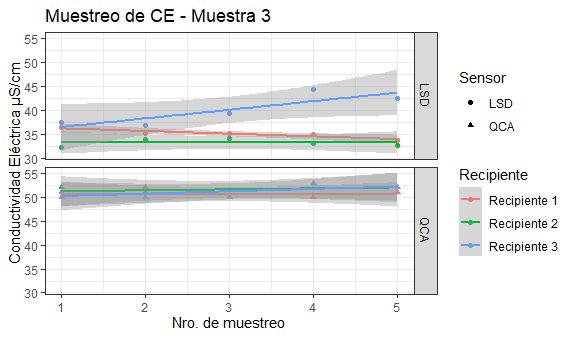
\includegraphics[width=0.75\linewidth]{Imagenes/cap4/CE_M3.png}
        \caption {Muestreo de conductividad el\'ectrica. }{\textbf{Fuente:}
        Elaboraci\'on Propia. }
        \label{fig:M3CE}
    \end{figure}

\subsubsection{Muestra 3. Sensor de pH}
%%%%% noooo
  \begin{table}[H]
        \protect\caption[Muestra 3: Agua de laguna]{Muestra 3: Agua de laguna.}
        \label{tab:TMuestra3}
        \centering
        \begin{tabular}{c c c}
            \hline
            \multicolumn{3}{c}{\textbf{Muestra 3: Agua de laguna.}} \\
             \hline
            \multicolumn{3}{c}{\textbf{Recipiente 1}} \\
            \hline
            \textbf{Lectura}&\textbf{LSD ($pH$)}&\textbf{Qca ($pH$)} \\
            \hline
            {1}& $6.302$&$6.99$ \\ 
            {2}& $6.285$&$6.98$ \\ 
            {3}& $6.318$&$6.96$ \\  
            {4}& $6.253$&$7.00$ \\ 
            {5}& $6.081$&$6.93$ \\
            \hline
            \multicolumn{3}{c}{\textbf{Recipiente 2}} \\
            \hline
            \textbf{Lectura}&\textbf{LSD ($pH$)}&\textbf{Qca ($pH$)} \\
            \hline
            {1}& $6.255$&$7.19$ \\ 
            {2}& $6.265$&$7.14$ \\ 
            {3}& $6.265$&$7.13$ \\  
            {4}& $6.138$&$7.10$ \\ 
            {5}& $6.138$&$7.20$ \\
            \multicolumn{3}{c}{\textbf{Recipiente 3}} \\
            \hline
            \textbf{Lectura}&\textbf{LSD ($pH$)}&\textbf{Qca ($pH$)} \\
            \hline
            {1}& $6.482$&$6.61$ \\ 
            {2}& $6.488$&$6.74$ \\ 
            {3}&$6.532$&$7.07$  \\  
            {4}& $6.538$&$7.01$ \\ 
            {5}& $6.522$&$7.20$ \\
            \hline
        \end{tabular}
        \vspace{5mm}
        \newline
        \hfill \textbf{Fuente: }Elaboración Propia.
    \end{table}

% Gráfico M3PH
\begin{figure}[H]
        \centering
        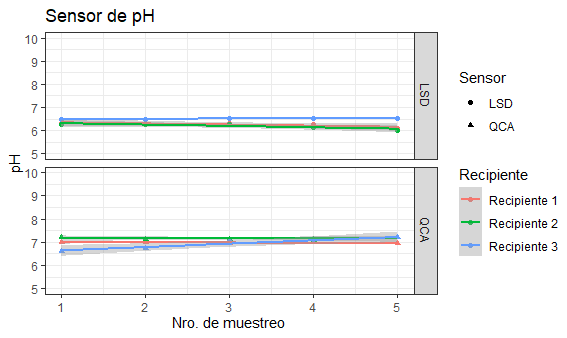
\includegraphics[width=0.75\linewidth]{Imagenes/cap4/pH_M3.png}
        \caption {Muestreo de pH. }{\textbf{Fuente:}
        Elaboraci\'on Propia. }
        \label{fig:M3PH}
\end{figure}

\subsection{An\'alsis de Datos. Muestra 3}

% Please add the following required packages to your document preamble:
% \usepackage{multirow}

\begin{table}[H]
\protect\caption[Muestra 3: Agua de laguna ]{Resumen de mediciones: Muestra 3.}
\label{tab:AnalisisM3}

\begin{tabular}{lccc|ccc}
\hline
Muestra 3 & 
\multicolumn{3}{c}{LSD}&
\multicolumn{3}{c}{QCA}\\ 
\textbf{\begin{tabular}[c]{@{}l@{}}An\'alisis de datos\end{tabular}} & \multicolumn{1}{c}{\begin{tabular}[c]{@{}c@{}}T \\ $^{\circ} C$\end{tabular}} & \multicolumn{1}{c}{pH}        & 
\begin{tabular}[c]{@{}c@{}}CE\\ $\mu S/cm$\end{tabular} & \multicolumn{1}{c}{\begin{tabular}[c]{@{}c@{}}T \\ $^{\circ} C$\end{tabular}} & \multicolumn{1}{c}{pH}        & 
\multicolumn{1}{c}{\begin{tabular}[c]{@{}c@{}}CE\\ $\mu S/cm$\end{tabular}}
\\ \hline
M\'inimo & \multicolumn{1}{c}{22.10}                            & \multicolumn{1}{c}{6.023} & 32.24                               & \multicolumn{1}{c}{21.80}                                       & 
\multicolumn{1}{c}{6.610} & 50.00   \\ M\'aximo                 & 
\multicolumn{1}{c}{22.90}                                       & 
\multicolumn{1}{c}{6.538} & 44.40                               & \multicolumn{1}{c}{22.90}                                       & 
\multicolumn{1}{c}{7.20}  & 53.00   \\ Promedio                 & 
\multicolumn{1}{c}{22.58}                                       & \multicolumn{1}{c}{6.316} & 36.12                               & \multicolumn{1}{c}{22.37}                                       & \multicolumn{1}{c}{7.017} & 51.13  \\ Desviación Est\'andar     & 
\multicolumn{1}{c}{0.291}                                       & \multicolumn{1}{c}{0.165} & 3.545                               & 
\multicolumn{1}{c}{0.354}                                       & 
\multicolumn{1}{c}{0.167}                                       & 
\multicolumn{1}{c}{1.125} \\ Varianza                           & \multicolumn{1}{c}{0.0845}                                      & \multicolumn{1}{c}{0.027} & 12.57                               & \multicolumn{1}{c}{0.125}                                       & 
\multicolumn{1}{c}{0.027}                                       & 
\multicolumn{1}{c}{1.267}  \\ Error Estándar                    & \multicolumn{1}{c}{0.075}                                       & \multicolumn{1}{c}{0.0426} & 0.915                              & 
\multicolumn{1}{c}{0.0914}                                      & 
\multicolumn{1}{c}{0.0431}                                      & 
\multicolumn{1}{c|}{0.290}  \\ 
\hline
\end{tabular}
\end{table}

En la tabla \ref{tab:AnalisisM3}, se puede observar algunos par\'ametros estad\'isticos calculados, a partir de los registros recolectados en el muestreo de los recipientes de la muestra 3, el cual arrojo los siguientes resultados. 
La desviaci\'on est\'andar m\'as elevada se registr\'o en el par\'ametro de conductividad el\'ectrica, siendo el mayor el registrado por el sensor de LSD, igual a 3.545 un  3.17\%  mayor a la desviación del sensor de QCA, en los resultados de  los otros par\'ametros, se registra un desviaci\'on parecidas siendo los menor en sensores de LSD,   . 
La varianza sigue la misma tendencia de la desviaci\'on est\'andar, la conductividad el\'ectrica presenta una mayor dispersi\'on. 
El error est\'andar, presenta valores bajos en todos los par\'ametros menores a 1, el cual sugiere que los valores recolectados son uniforme y se encuentran cerca de la media. 
Los valores mínimos recolectados en el caso de la temperatura presentan una deferencia de 0,3 $ ^{\circ}C$ siendo 21.3$ ^{\circ}C$ la menor lectura registrada por el sensor de QCA, en el caso del pH la diferencia entre los mínimos fue de 0,587 pH, siendo 6,023 pH la menor lectura registrada por el sensor de LSD, la m\'inima conductividad el\'ectrica registrado fue de 32,24 $\mu S/cm$ con una diferencia de 17,76 $\mu S/cm$ con respecto al sensor de QCA. 
Los valores m\'aximo recolectados en el caso de la temperatura no presentaron  deferencia siendo 22,90 $ ^{\circ}C$ la  lectura registrada por los sensores, en el caso del pH la diferencia entre los m\'aximos fue de 0.662 pH, siendo 7.2 pH la mayor lectura registrada por el sensor de QCA, la conductividad el\'ectrica m\'as alta registrada fue de 53 $\mu S/cm$ con con una diferencia de 8.6 $\mu S/cm$ con respecto a la mayor lectura registrada en el sensor QCA.
El promedio de las mediciones fueron cercanas con una diferencia de 9 $\%$ en el caso del pH, siendo el promedio de los datos de pH registrado por el sensor de QCA 7,017 pH contra el promedio de pH registrado por el sensor LSD igual a 6.316 pH, en el caso de los resultados promedios registrados de la temperatura la diferencia entre los resultados fue menor al 0.93$\%$ siendo la temperatura promedio del sensor LSD igual a 22.58$ ^{\circ}C$ y la temperatura promedio del sensor de QCA igual a 22.37$^{\circ}C$, los promedio de las mediciones de los sensores de conductividad eléctrica entre los sensores tienen diferencia de 29.35 $\%$, siendo el promedio de los datos de CE registrado por el sensor de QCA 51.13 contra el promedio de CE registrado por el sensor LSD igual a 36.12 $\mu S/cm$.
En este an\'alisis de datos correspondiente a la muestra 3, se observan los mismos patrones, los resultados finales con valores cercanos, con un margen de diferencia menor al 7\% entre ambos sensores de ph - T y menor al 23.35 \% en el sensor de CE.

\begin{table}[H]
\caption{Relaci\'on entre los equipos de sensores}
\label{tab:VaCoM3}
\centering
\begin{tabular}{llll} 
\toprule
& T   &  pH    & CE \\
\midrule
Covarianza  & 0.05483 & 0.0073 & 0.157                \\
Correlación & 0.5483& 0.3782 & 0.628        \\
\bottomrule
\end{tabular}
\\ \textbf{Fuente: }Elaboración Propia.
\end{table}  

En un an\'alisis de la tabla \ref{tab:VaCoM2}, donde se encuentran los resultados de covarianza y correlación de las muestras, en el caso de la temperatura, conductividad el\'ectrica y pH se obtuvieron unos valores de covarianzas positivas el cual indica que ambas lecturas varían en la misma dirección, as\'i mismo en los tres par\'ametros se obtuvieron correlaciones positivas menores a 1, refleja que se da una correlación positiva entre sí, la media varía en la misma dirección con el factor del valor del coeficiente de correlación. Luego de analizar los resultados obtenidos en el caso de la muestra 3, se puede concluir que ambos sensores presentan lecturas cercanas,relacionadas entre s\'i, con baja dispersi\'on. 

% resumen de mediciones

%Estadistica de mediciones

\section{Pruebas de campo}
Las pruebas en campo se realizaron con el fin de verificar el comportamiento de la sonda y sistemas en un entorno de trabajo real. 
Se realizaron varias pruebas de campos en el lago Ypakarai, los cuales ayudaron a mejorar el dise\~no final, desde el punto de hardware y software, alguna de las mejoras fueron,laincorporaci\'on de una estructura interna de fijado por la base de la sonda, a modo de sostener y mantener ordenado todos los elementos electr\'onicos, evitando con esto que se puedan da\~nar por su manipulaci\'on, incorporaci\'on de un o-ring para mejorar el hermetismo e impedir el ingreso de l\'iquidos, ya que luego de las primeras pruebas se detectaron filtraciones provenientes de la rosca principal uni\'on base-anillo,para la publicaci\'on remota, se agreg\'o al c\'odigo principal, rutinas multi hilos, para cuando la sonda pierda conexi\'on a internet no se pierdan estos paquetes durante, y unan vez recuperada la conexi\'on se env\'ien todos los hilos.

\begin{figure}[H]
     \centering
     \begin{subfigure}[b]{0.65\textwidth}
         \centering
         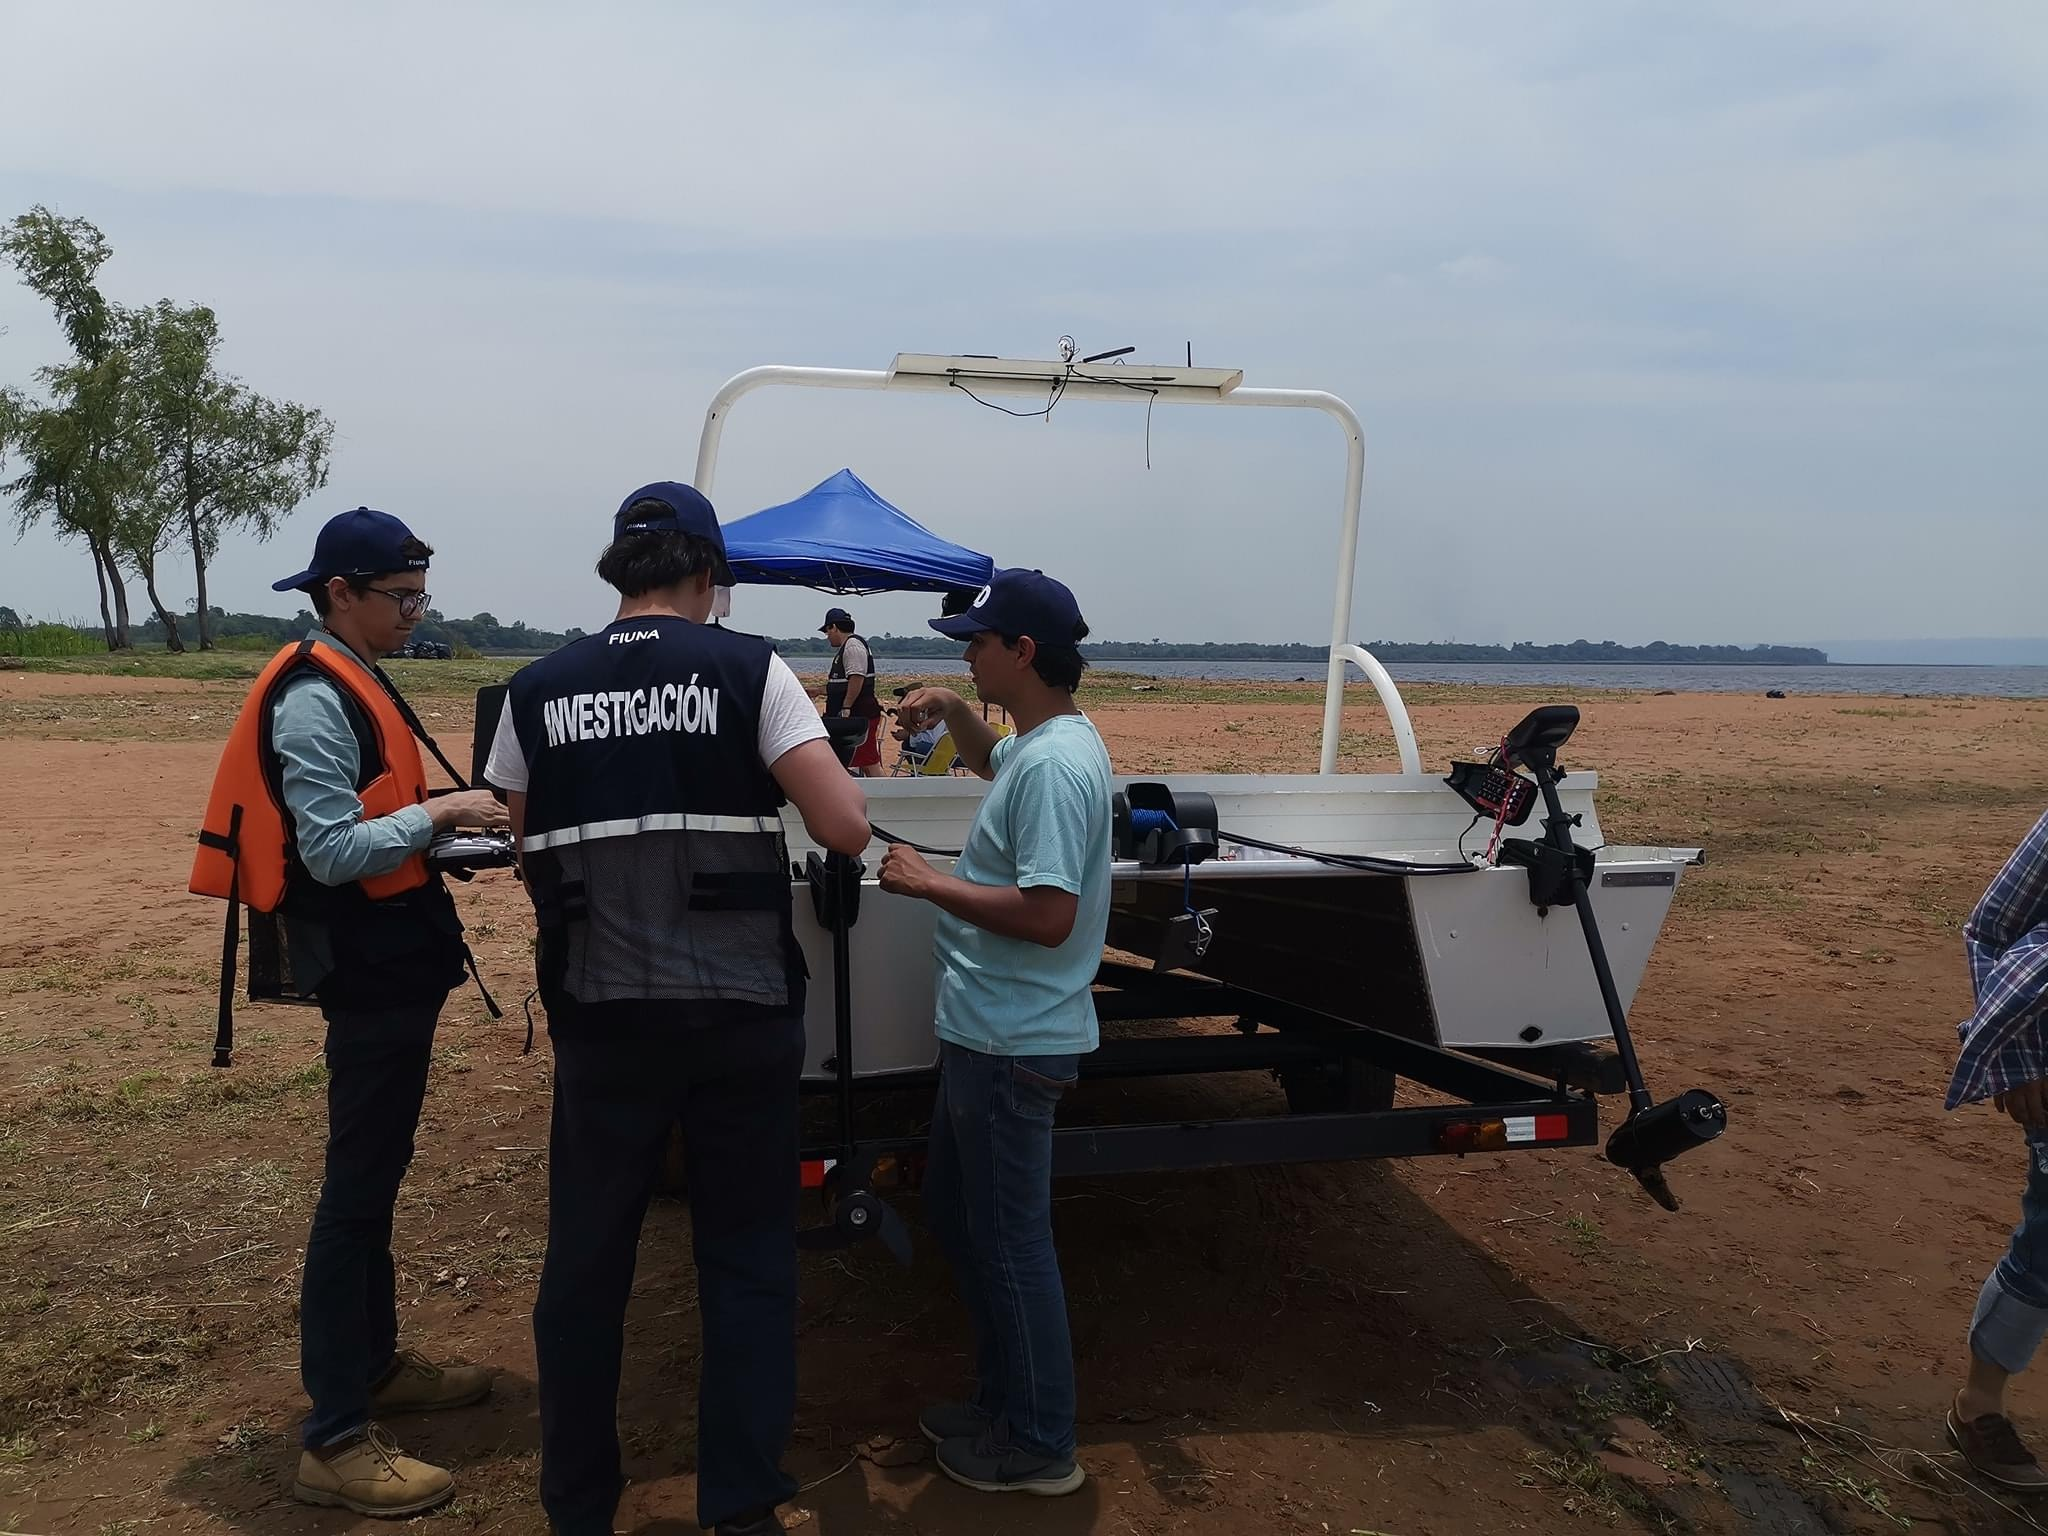
\includegraphics[width=\textwidth]{Imagenes/cap4/PruebaCampo.jpeg}
         \caption{Preparaci\'on del ASV.}
         \label{fig:PreparacionASV}
     \end{subfigure}
     \hfill
     \begin{subfigure}[b]{0.3\textwidth}
         \centering
         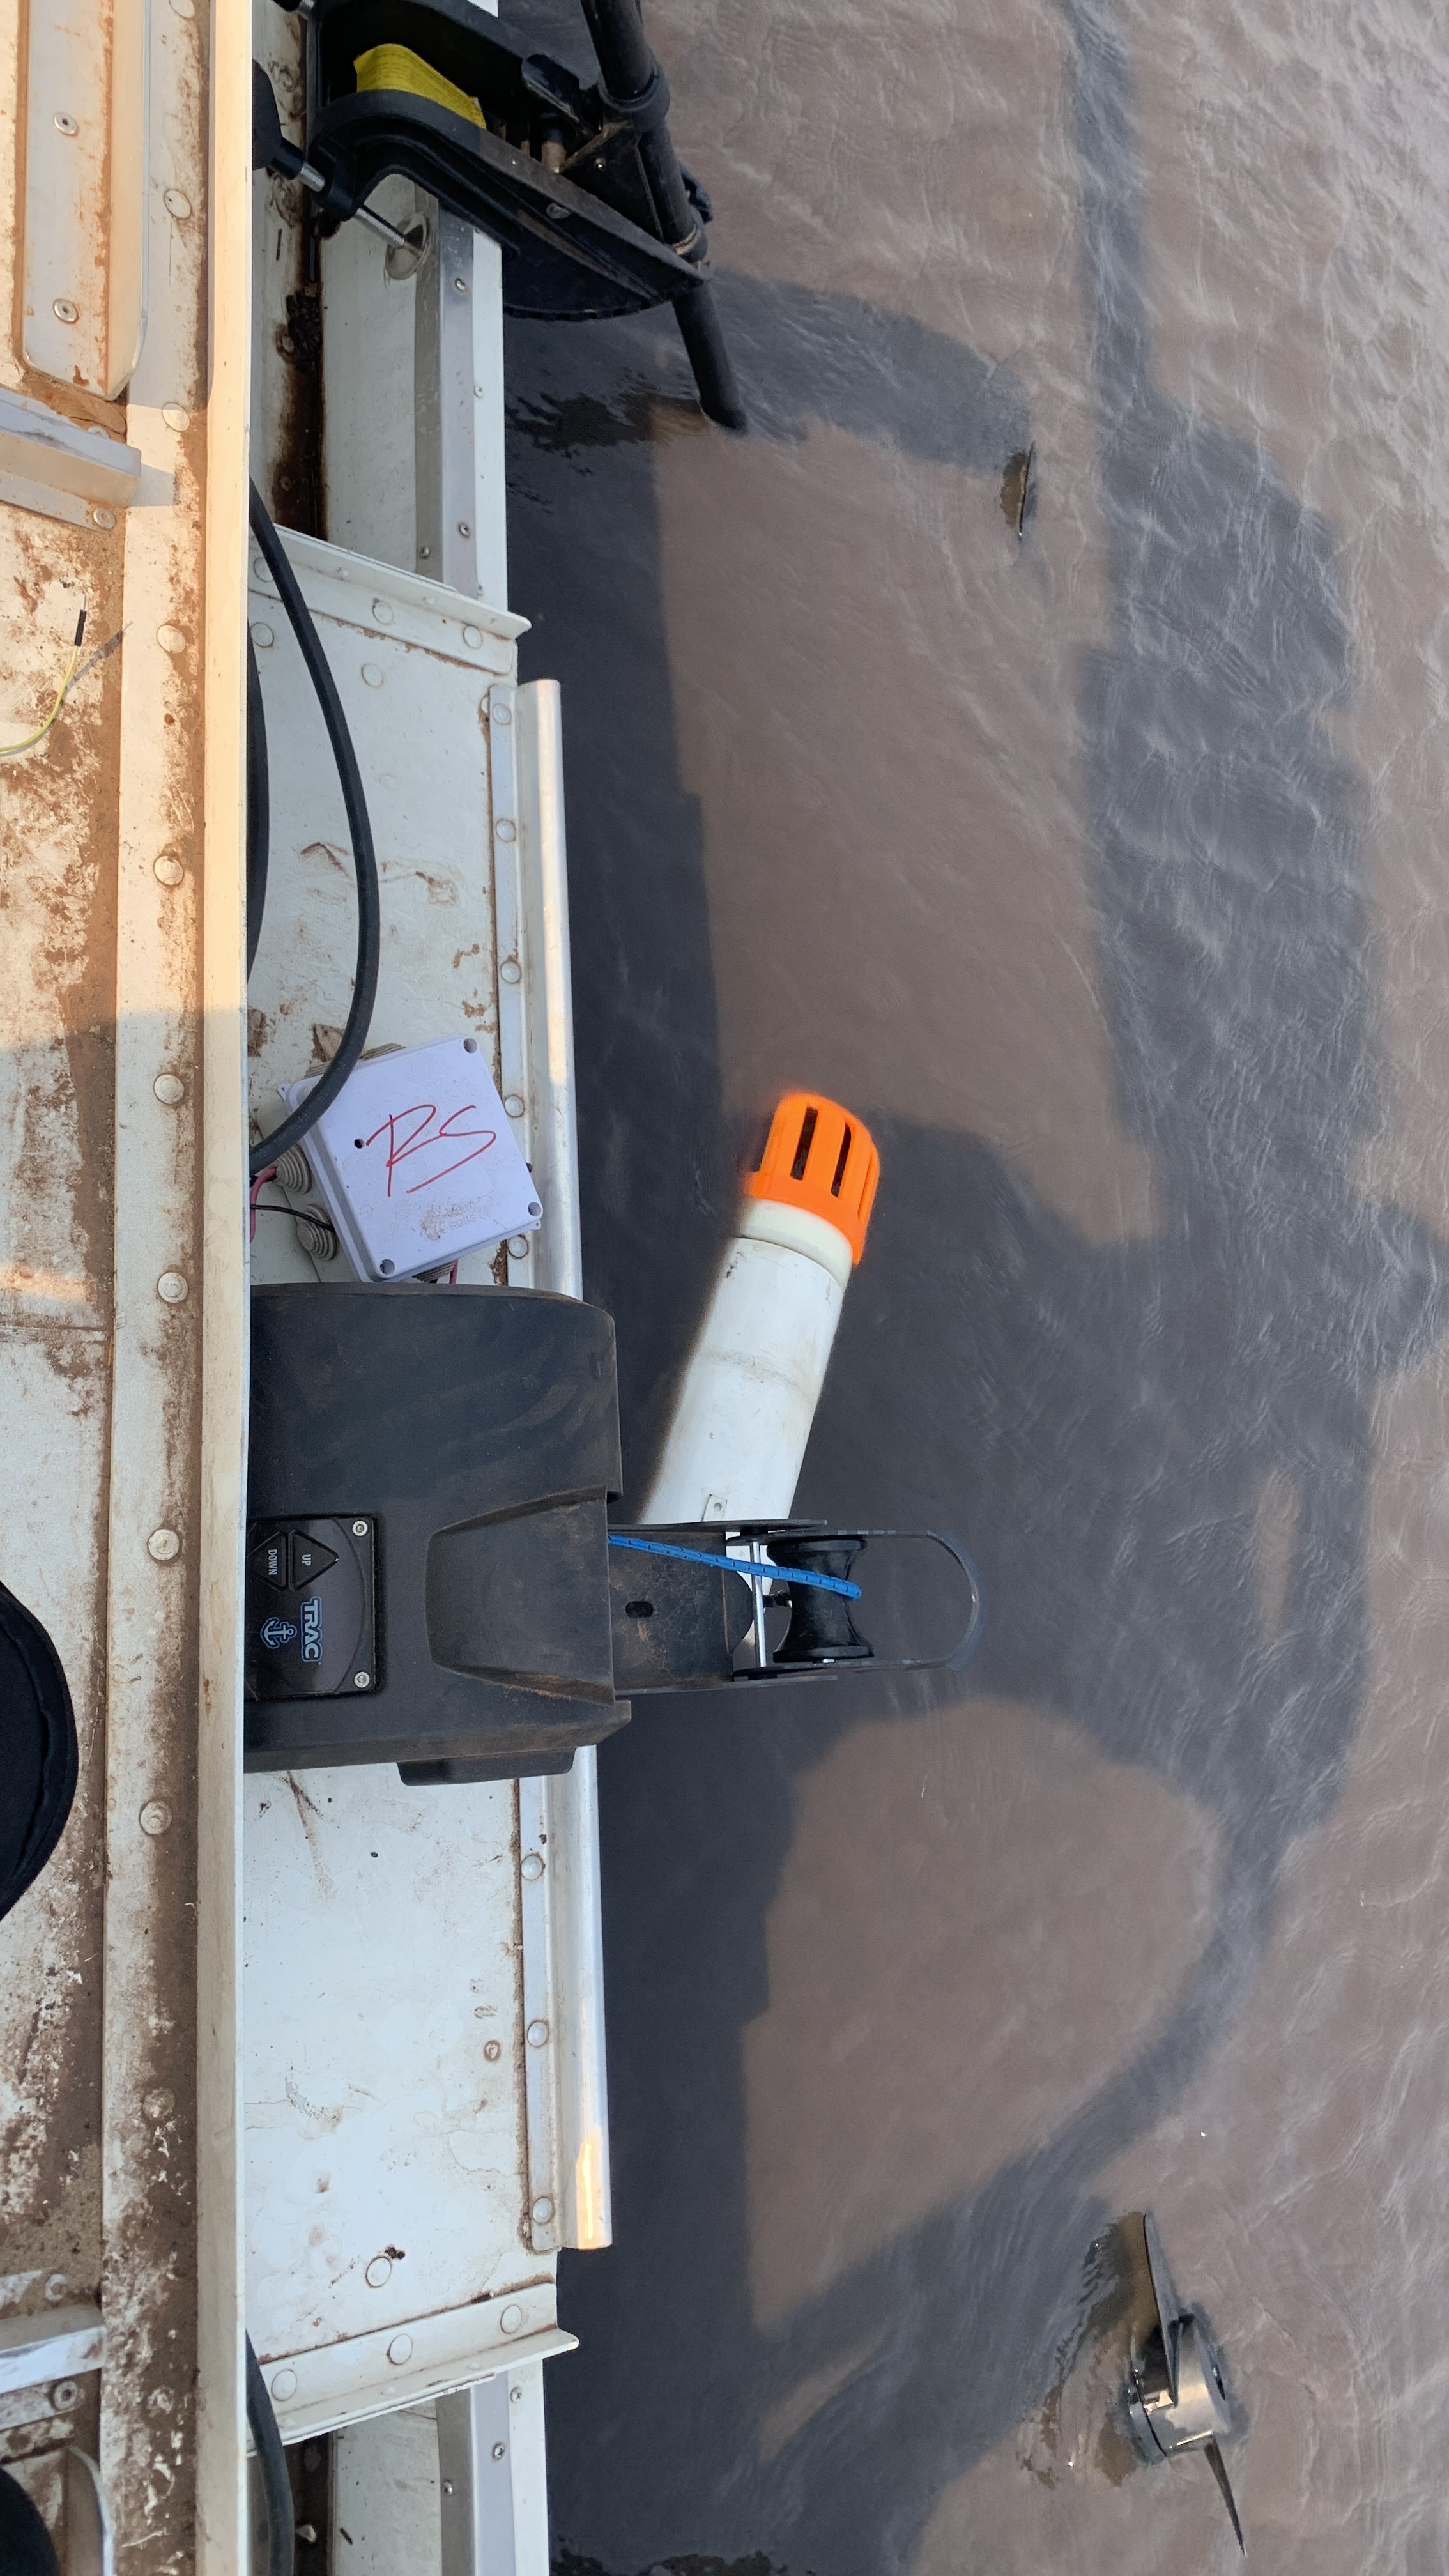
\includegraphics[width=\textwidth]{Imagenes/cap4/PruebaCampo1.JPG}
         \caption{Sonda instalada en el ASV.}
         \label{fig:SondaASV}
     \end{subfigure}
     \hfill
    \caption{Prueba de campo - Lago Ypakarai}
    \label{fig:PruebaCampo}
\end{figure}


\subsection{Muestreo de pH. Prueba de Campo}

\begin{figure}[H]
        \centering
        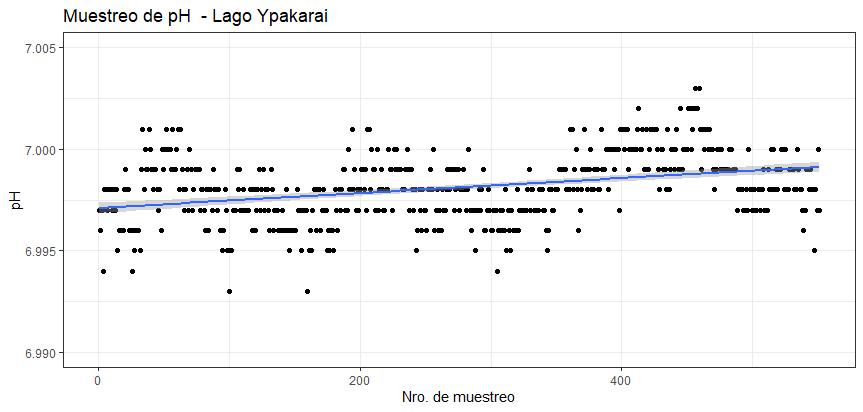
\includegraphics[width=0.75\linewidth]{Imagenes/cap4/pHLago.png}
        \caption {Muestreo de pH, lago Ypakarai. }{\textbf{Fuente:}
        Elaboraci\'on Propia. }
        \label{fig:Lago_ph}
\end{figure}

La Resoluci\'on. SEAM N$ ^{\circ}$ 222/02 estable un l\'imite inferior y superior igual a 6 y 9 respectivamente.Durante esta campa\~na todos los puntos se encuentran acorde a la normativa.
En la tabla \ref{table:Lago_ph} se presenta un an\'alisis comparativo de los valores obtenidos para el par\'ametro pH correspondientes a la prueba de campo  realizada.

\begin{table}[H]
\centering
\caption{Prueba de campo. Estadísticas descriptivas – ph}
\label{table:Lago_ph}
\begin{tabular}{lrrrr}
\toprule & 
\multicolumn{3}{r}{Rango} \\ \cline{4-5} & 
Muestras & Promedio & Mínimo & Máximo \\
\midrule
Prueba de campo  &      472 &      7.0 &  6.993 &  7.003 \\
\bottomrule
\end{tabular}
\end{table}
Se realizaron 472 mediciones en todo el recorrido, los valores recolectados de potencial de hidr\'ogeno que oscilan en un intervalo entre 6.993 y 7.003.
En la tercera \cite{3er_Cemit} y cuarta \cite{4to_Cemit} campaña de muestreo del “Monitoreo de Calidad de Agua por Campañas de Muestreo en el Lago Ypacaraí 2019 -2021, correspondientes al periodo de la prueba de campo, realizado por CEMIT-UNA, segun contrato ITAIPÚ/UNA No. 4500054462/2019, se documentan promedios de pH que oscilaron entre 6.0 y 7.98. 
Se verifica que par\'ametro recolectados en esta campa\~na se encuentra dentro del intervalo de valores.

\subsection{Muestreo de CE. Prueba de Campo}

\begin{figure}[H]
        \centering
        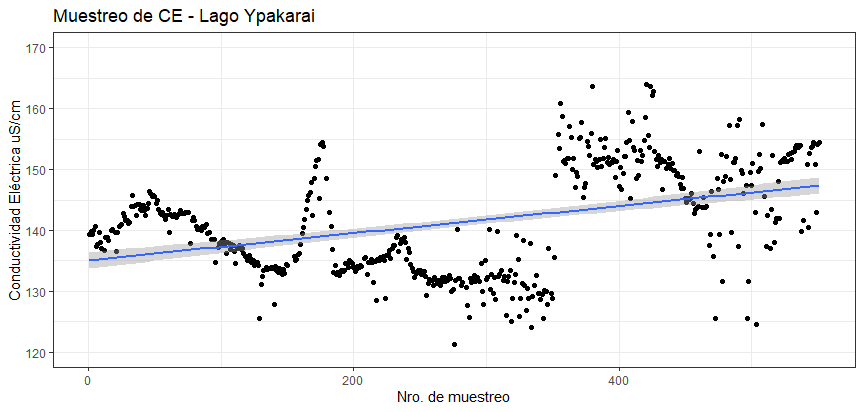
\includegraphics[width=0.75\linewidth]{Imagenes/cap4/CE_lago.png}
        \caption {Muestreo de CE, lago Ypakarai. }{\textbf{Fuente:}
        Elaboraci\'on Propia. }
        \label{fig:Lago_ce}
\end{figure}

Para aguas de Clase 2 la Resoluci\'on 222/02 no estable ningún l\'imite para el par\'ametro evaluado; se toma como referencia el l\'mite de 1250 $\mu S/cm$ establecido en el Anexo X de la ley 1614/2000 en cual Ley General Del Marco Regulatorio y Tarifario Del Servicio De Agua Potabley Alcantarillado Sanitario. Todas las determinaciones realizadas en la campa\~na se encuentran en conformidad con la normativa de referencia.
En la tabla \ref{table:Lago_ce} se presenta un an\'alisis comparativo de los valores obtenidos para el par\'ametro CE correspondientes a la prueba de campo  realizada.

\begin{table}[H]
\centering
\caption{Prueba de campo. Estadísticas descriptivas – ce}
\label{table:Lago_ce}
\begin{tabular}{lrrrr}
\toprule& 
\multicolumn{3}{r}{Rango} \\  \cline{4-5}& 
Muestras & Promedio & Mínimo & Máximo \\
\midrule
Prueba de campo  &      472 &   137.65 &   4.62 &  163.6 \\
\bottomrule
\end{tabular}
\end{table}

Se realizaron 472 mediciones en todo el recorrido, los valores recolectados de conductividad el\'ectrica que oscilan en  un intervalo entre 4.62 $\mu S/cm$ y 163.6 $\mu S/cm$, en promedio 137.65 $\mu S/cm$.
En la tercera \cite{3er_Cemit} y cuarta \cite{4to_Cemit} campaña de muestreo del “Monitoreo de Calidad de Agua por Campañas de Muestreo en el Lago Ypacaraí 2019 -2021, correspondientes al periodo de la prueba de campo, realizado por CEMIT-UNA, segun contrato ITAIPÚ/UNA No. 4500054462/2019, se documentan promedios de CE que oscilaron entre $156 \mu S/cm$ y $601 \mu S/cm$. 
Se verifica que los datos del par\'ametro, recolectados en esta campa\~na se encuentra dentro del intervalo de valores.

\subsection{Muestreo de OD. Prueba de Campo}

\begin{figure}[H]
        \centering
        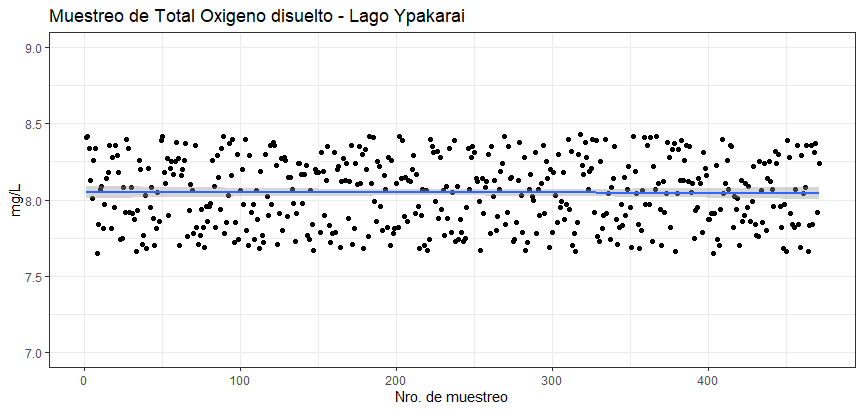
\includegraphics[width=0.75\linewidth]{Imagenes/cap4/OD_Lago Ypakarai.png}
        \caption {Muestreo de OD, lago Ypakarai.}{\textbf{Fuente:}
        Elaboraci\'on Propia. }
        \label{fig:Lago_od}
\end{figure}

La Resoluci\'on SEAM 222/02 establece que el ox\'igeno disuelto en aguas de clases 2 debe ser  $> 5 mg O_2/L$. Todas las determinaciones realizadas en la campa\~na se encuentran en conformidad con la normativa de referencia.
En la tabla \ref{table:Lago_od} se presenta un an\'alisis comparativo de los valores obtenidos para el par\'ametro OD correspondientes a la prueba de campo  realizada.

\begin{table}[H]
\centering
\caption{Prueba de campo. Estadísticas descriptivas – OD}
\label{table:Lago_od}
\begin{tabular}{lrrrr}
\toprule
          & \multicolumn{3}{r}{Rango} \\ \cline{4-5}
          & Muestras & Promedio & Mínimo & Máximo \\
\midrule
Prueba de campo  &      472 &     8.05 &   7.65 &   8.43 \\
\bottomrule
\end{tabular}
\end{table}

Se realizaron 472 mediciones en todo el recorrido, los valores recolectados de oxigeno disuelto que oscilan en  un intervalo entre 7.65   y 8.43 $mg/L$, en promedio 8.05 $mg/L$.
En la tercera \cite{3er_Cemit} y cuarta \cite{4to_Cemit} campaña de muestreo del “Monitoreo de Calidad de Agua por Campañas de Muestreo en el Lago Ypacaraí 2019 -2021, correspondientes al periodo de la prueba de campo, realizado por CEMIT-UNA, segun contrato ITAIPÚ/UNA No. 4500054462/2019, se documentan promedios de CE que oscilaron entre 7.85 $mg/L$ y 8.9 $mg/L$. 
Se verifica que los datos del par\'ametro, recolectados en esta campa\~na se encuentra dentro del intervalo de valores.

\subsection{Muestreo de OPR. Prueba de Campo}

\begin{figure}[H]
        \centering
        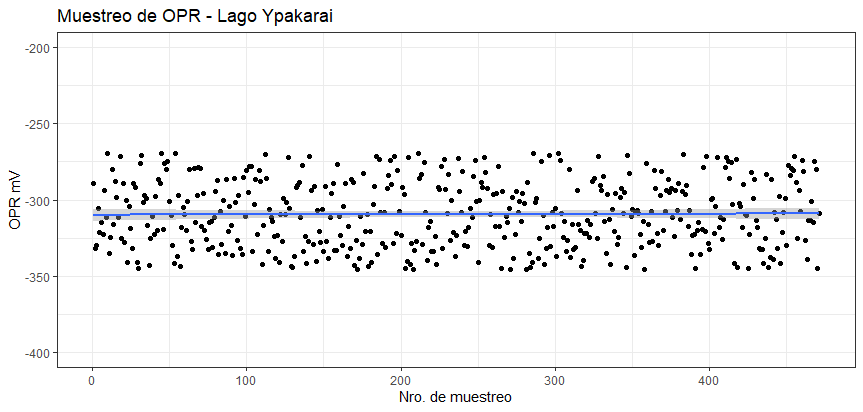
\includegraphics[width=0.75\linewidth]{Imagenes/cap4/OPR_LAGO.png}
        \caption {Muestreo de OPR, lago Ypakarai. }{\textbf{Fuente:}
        Elaboraci\'on Propia. }
        \label{fig:Lago_opr}
\end{figure}
La Resoluci\'on. SEAM N$ ^{\circ}$ 222/02 no define un valor límite para OPR La Organización Mundial de la Salud adoptó en 1972 la medida del POTENCIAL REDOX como la medida más fiable para medir la calidad sanitaria del agua potable, estableciendo en \cite{OPR_10665-39989} el valor 650mV como valor adecuado para el agua potable.
En la tabla \ref{table:Lago_temp} se presenta un an\'alisis comparativo de los valores obtenidos para el par\'ametro OPR correspondientes a la prueba de campo realizada. 
\begin{table}[H]
\centering
\caption{Prueba de campo. Estadísticas descriptivas – OPR}
\label{table:Lago_opr}
\begin{tabular}{lrrrr}
\toprule
          & \multicolumn{3}{r}{Rango} \\  \cline{4-5}
          & Muestras & Promedio & Mínimo & Máximo \\
\midrule
Prueba de campo  &      472 &  -309.43 & -345.7 & -269.1 \\
\bottomrule
\end{tabular}
\end{table}

Se realizaron 472 mediciones en todo el recorrido, los valores recolectados de oxigeno disuelto que oscilan en  un intervalo entre -259.1 $mV$ y -345.7 $mV$, en promedio -309.4 $mV$.

\subsection{Muestreo de T. Prueba de Campo}

\begin{figure}[H]
        \centering
        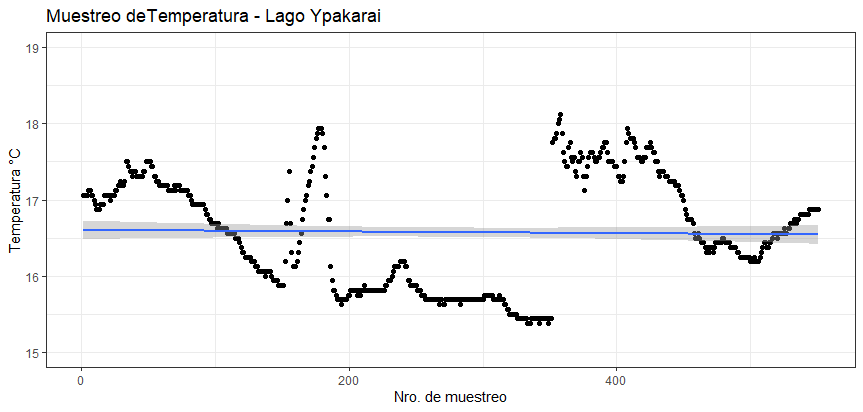
\includegraphics[width=0.75\linewidth]{Imagenes/cap4/Temp_lago.png}
        \caption {Muestreo de T, lago Ypakarai. }{\textbf{Fuente:}
        Elaboraci\'on Propia. }
        \label{fig:Lago_temp}
\end{figure}

La Resoluci\'on. SEAM N$ ^{\circ}$ 222/02 no define un valor límite para la temperatura de las aguas de Clase 2; solo para el vertido de efluentes a cuerpos receptores se establece un valor límite de 40$ ^{\circ}$C.
En la tabla \ref{table:Lago_temp} se presenta un an\'alisis comparativo de los valores obtenidos para el par\'ametro T correspondientes a la prueba de campo  realizada.

\begin{table}[H]
\centering
\caption{Prueba de campo. Estadísticas descriptivas – temp}
\label{table:Lago_temp}
\begin{tabular}{lrrrr}
\toprule
          & \multicolumn{3}{r}{Rango} \\ \cline{4-5}
          & Muestras & Promedio & Mínimo & Máximo \\
\midrule
Prueba de campo  &      472 &    16.51 & 15.375 & 18.125 \\
\bottomrule
\end{tabular}
\end{table}

Se realizaron 472 mediciones en todo el recorrido, los valores recolectados de temperatura que oscilan en  un intervalo entre 15.37 $ ^{\circ}$C y 18.12 $ ^{\circ}$C, en promedio 16.51 $^{\circ}$C .
En la tercera \cite{3er_Cemit} y cuarta \cite{4to_Cemit} campaña de muestreo del “Monitoreo de Calidad de Agua por Campañas de Muestreo en el Lago Ypacaraí 2019 -2021, correspondientes al periodo de la prueba de campo, realizado por CEMIT-UNA, segun contrato ITAIPÚ/UNA No. 4500054462/2019, se documentan promedios de T que oscilaron entre 19.7 $ ^{\circ}$C y 26.2 $ ^{\circ}$C. 
Se verifica que los datos del par\'ametro, recolectados en esta campa\~na no se encuentra dentro del intervalo de valores.

\subsection{Muestreo de TDS. Prueba de Campo}

\begin{figure}[H]
        \centering
        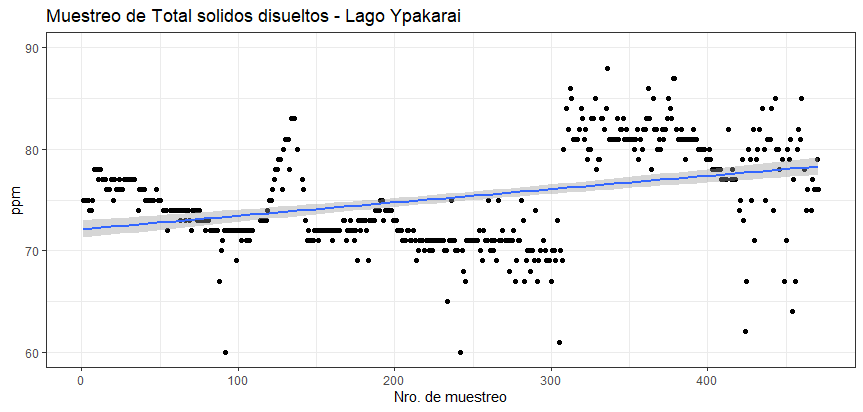
\includegraphics[width=0.75\linewidth]{Imagenes/cap4/TDS LagoYpakarai.png}
        \caption {Muestreo de TDS, lago Ypakarai. }{\textbf{Fuente:}
        Elaboraci\'on Propia. }
        \label{fig:Lago_tds}
\end{figure}

La Resoluci\'on SEAM 222/02 establece que el total de solidos disuelto en aguas de aguas del territorio nacional ser menor a  500$ mg /L$. Todas las determinaciones realizadas en la campa\~na se encuentran en conformidad con la normativa de referencia.
En la tabla \ref{table:Lago_tds} se presenta un an\'alisis comparativo de los valores obtenidos para el par\'ametro TDS correspondientes a la prueba de campo  realizada.

\begin{table}[H]
\centering
\caption{Prueba de campo. Estadísticas descriptivas – tds}
\label{table:Lago_tds}
\begin{tabular}{lrrrr}
\toprule
          & \multicolumn{3}{r}{Rango} \\ \cline{4-5}
          & Muestras & Promedio & Mínimo & Máximo \\
\midrule
Prueba de campo  &      472 &    73.86 &    2.0 &   88.0 \\
\bottomrule
\end{tabular}
\end{table}

\subsubsection{Resumen del an\'alsis de Datos. Prueba de Campo}
A continuaci\'on se presenta un resumen de todos los datos obtenidos.
El muestreo se hizo durante el desplazamiento en un circuito cerrado partiendo de la playa municipal de San Bernardino, pasando por el centro del lago Ypakarai  y la desembocadura del arrollo Piray\'u, tal como se puede observar en la figura \ref{fig:ruta}, el muestreo inicio a las 10:00hs hasta las 12:25hs, durante este periodo se registraron 471 (cuatrocientos setenta y uno) muestras, en intervalos aproximados de 25 segundos, los par\'ametros  recolectados durante el muestreo de pH, conductividad el\'ectrica, ox\'igeno disuelto, total de s\'olidos disueltos, potencial \'oxido reducci\'on y temperatura, los datos de georeferenciaci\'on fueron prove\'idos por el ASV en cada punto de muestreo.
\begin{figure}[H]
        \centering
        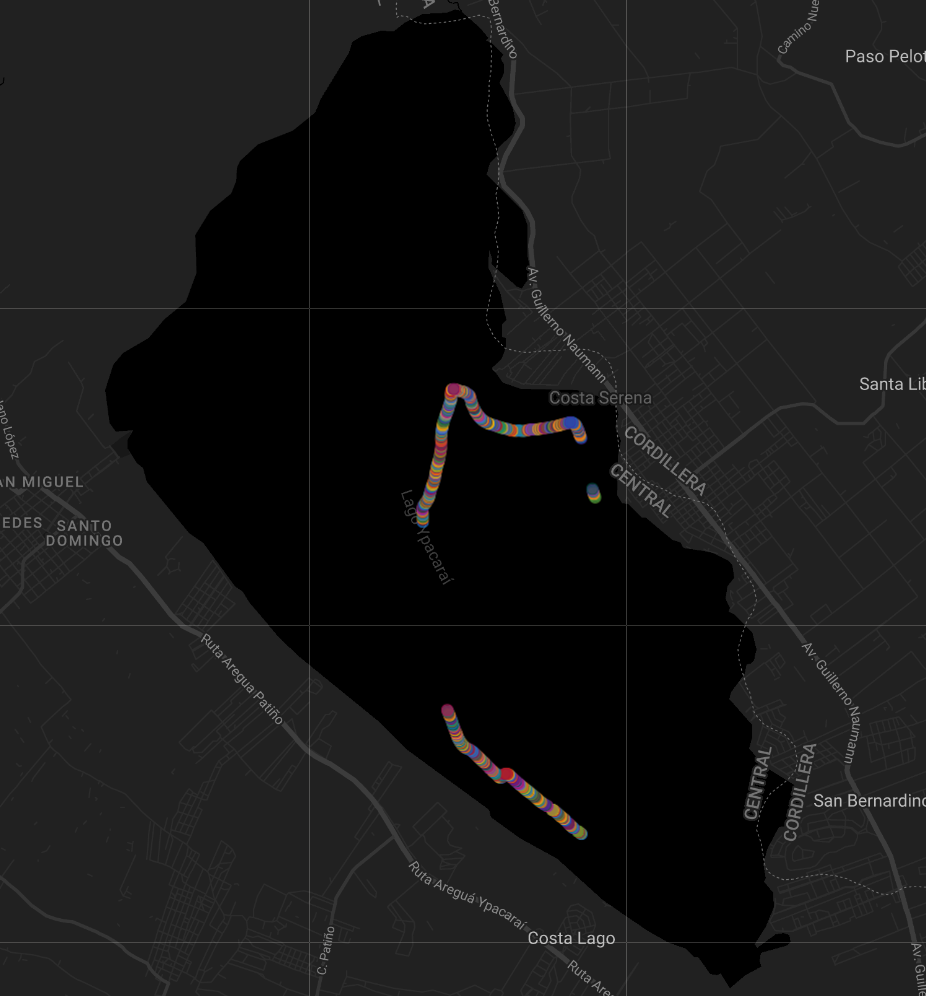
\includegraphics[scale=0.7]{Imagenes/cap4/Recorrido.png}
        \caption {Ruta de muestreo. }{\textbf{Fuente:}
        Elaboraci\'on Propia. }
        \label{fig:ruta}
\end{figure}

En la tabla \ref{tab:datos Lago}, se presenta los rsultados de unos an\'alisis estadísticos descriptivos correspondientes a todos los par\'ametros de la prueba de campo realizada.

\begin{table}[H]
\caption{Muestreo lago Ypakarai. Resumen}
\label{tab:datos Lago}
\begin{tabular}{lllllll} \hline& 
T  $^{\circ}C$ & $pH$     & CE $\mu S/cm$ & TDS $ppm$ & OPR $mV$ & OD $mgL/$  \\ \hline
M\'inimo & 15.37 & 6.993 & 4.62 & 2    & -345.70  & 7.65     \\
M\'aximo & 18.12 & 7.0   & 163.6    & 88    & -269.10  & 8.43 \\
Promedio & 16.51  & 6.99 & 137.65 & 73.85 & -309.42  & 8.047 \\
Desv. est. & 0.748 & 0.0016   & 17.50   & 9.46     & 21.634   & 0.22     \\
Varianza                & 0.56           & 0.000003 & 777.14        & 225.07    & 468.03   & 0.050296 \\
Error est.               & 0.034 & 0.000076 & 1.283154 & 0.690544 & 0.995786 & 0.010323 \\
\hline
\end{tabular}
\end{table}
Los temperatura maxima registrada fye de 18.12 $^o$C, el potencial de hidrigeno maximo fue de 7pH, el valor maximo de la conductividad electrica fue de 163.6 $\mu S/cm$, el valor maximo de TDS fue 88ppm, en el caso de OPR fue -269.10 $mV$ y el oxigeno disuelto macimo resgrado fue 0.22 $mg/L$.
Se puede apreciar que los sensores de temperatura, pH, y oxigeno disuelto presentaron resultados de desviación estándar mas bajos, por lo tanto menos disperso. En el caso de la conductividad eléctrica, total de solidos disueltos y opr, presentaron valores de desviación estándar mas altas, por lo que se concluye de su comportamiento mas disperso.
El error estándar calculado es bajo para todas las medicines. 
Todo los datos obtenidos se encuentran en el intervalo de valores obtenidos en otras campa\~nas de muestreo como ser lo desarrollados por CEMIT- Itaipu \cite{3er_Cemit}\cite{4to_Cemit}, realizados en un periodo cercano a esta prueba de campo, y también se encuentran dentro de los valores obtenidos en \cite{lopez_moreira_m_eutrophication_2018}, donde se analizaron algunos de estos parámetros.  

\section{Interfaz de monitoreo}
La interfaz gr\'afica fue desarrollada con el objetivo de ofrecer una pre visualizaci\'on de los datos recolectados en tiempo de ejecucion, sin tener que acceder directamente a la base de datos, que sea de f\'acil uso y compatible con la mayor cantidad de dispositivos posibles.
Con la tecnolog\'ia NodeRed, fue posible instalar la interfaz gr\'fica mediantes nodos y con el protocolo de comunicaci\'on  MQTT lograr capturar los datos enviados por los t\'opicos antes  establecidos, \appendixautorefname{appendix: Topicos}
La interfaz gr\'afica es multi plataforma, compatibles con todos los sistemas operativos m\'oviles como de escritorio, ya que al ser una aplicaci\'on web instalada en servidores, es compatible con cualquier dispositivo que tenga instalado alg\'un navegador web donde se ejecutarse. En la figura \ref{fig:Monitoreo} se puede apreciar la interfaz gráfica fue instalada en el raspberry de la sonda y en la sala de monitoreo del laboratorio de sistemas distribuidos de fiuna ubicado en CITEC. 
\begin{figure}[H]
        \centering
        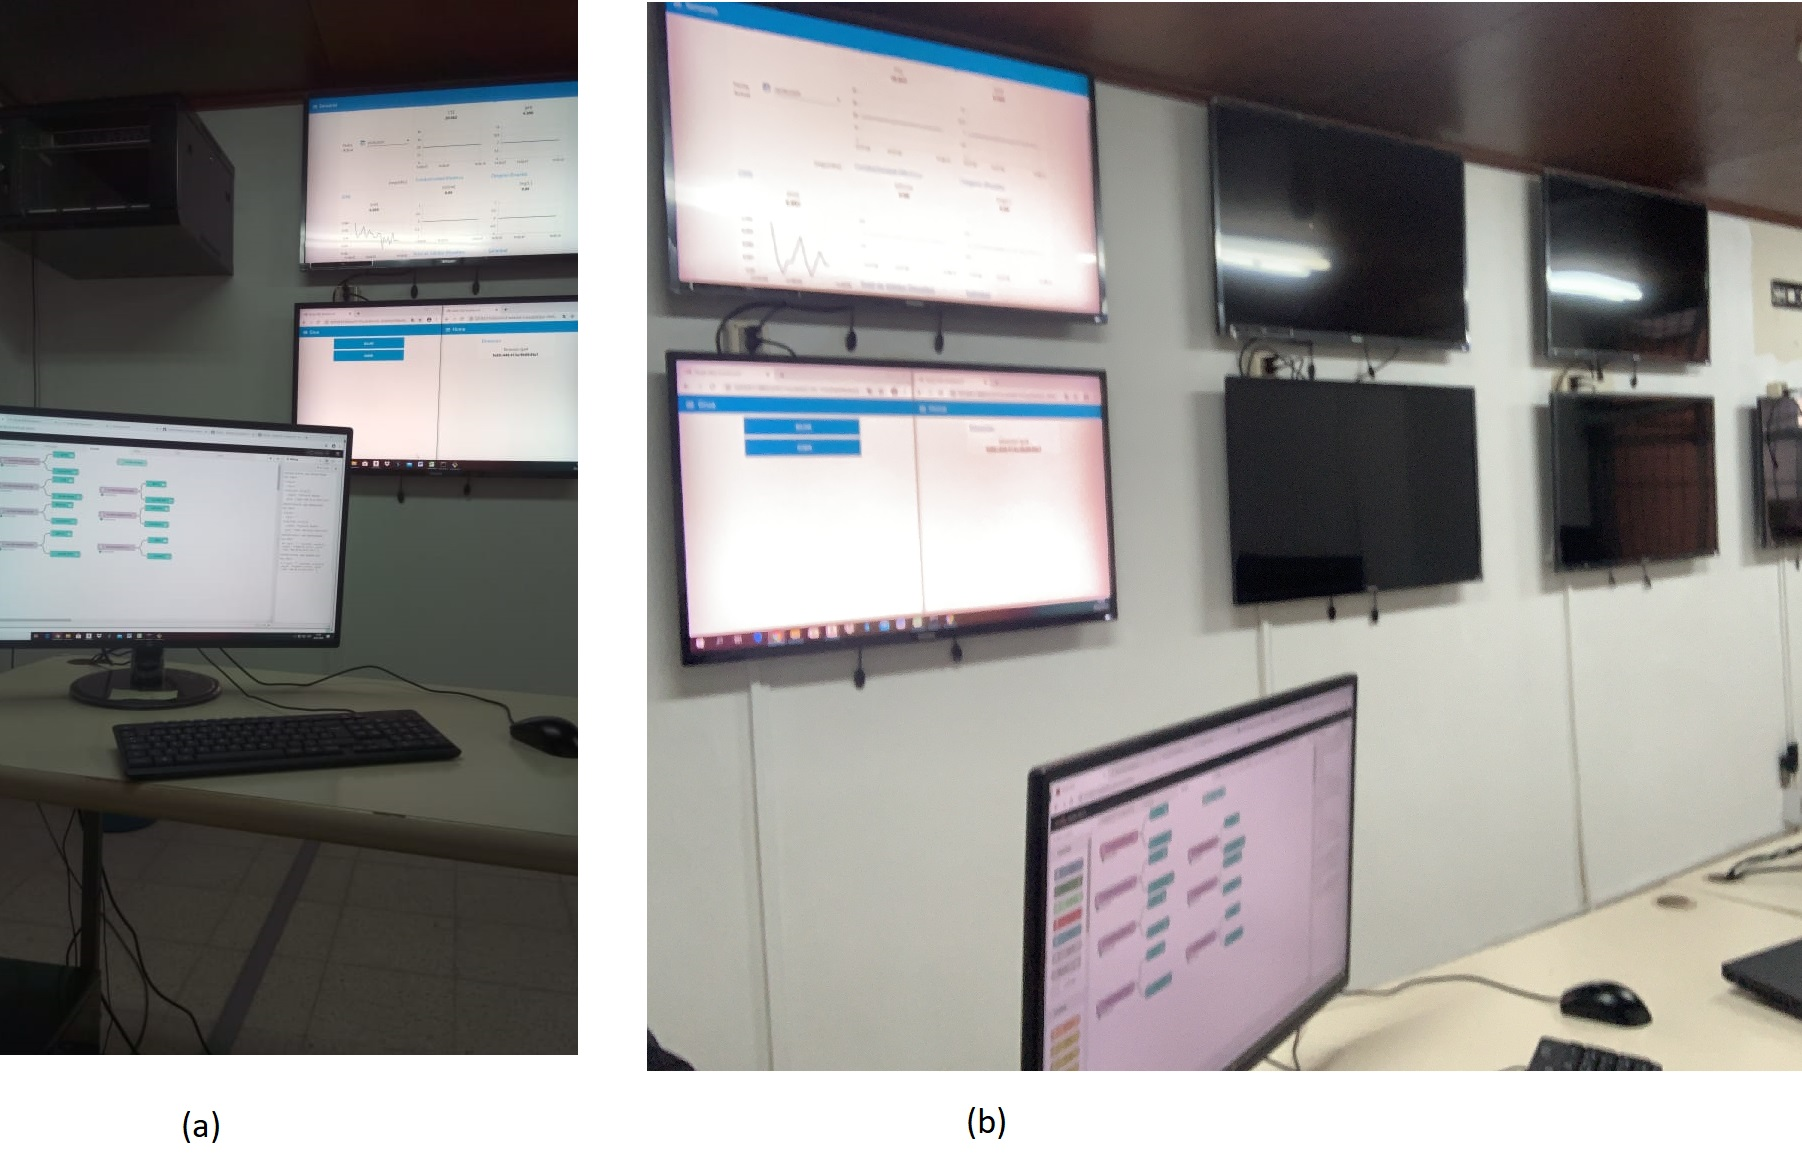
\includegraphics[scale=0.7]{Imagenes/cap4/SalaMonitoreo.jpg}
        \caption {Implementaci\'on de interfaz en la sala de monitoreo CITEC. }{\textbf{Fuente:}
        Elaboraci\'on Propia. }
        \label{fig:Monitoreo}
\end{figure}


\begin{figure}[H]
        \centering
        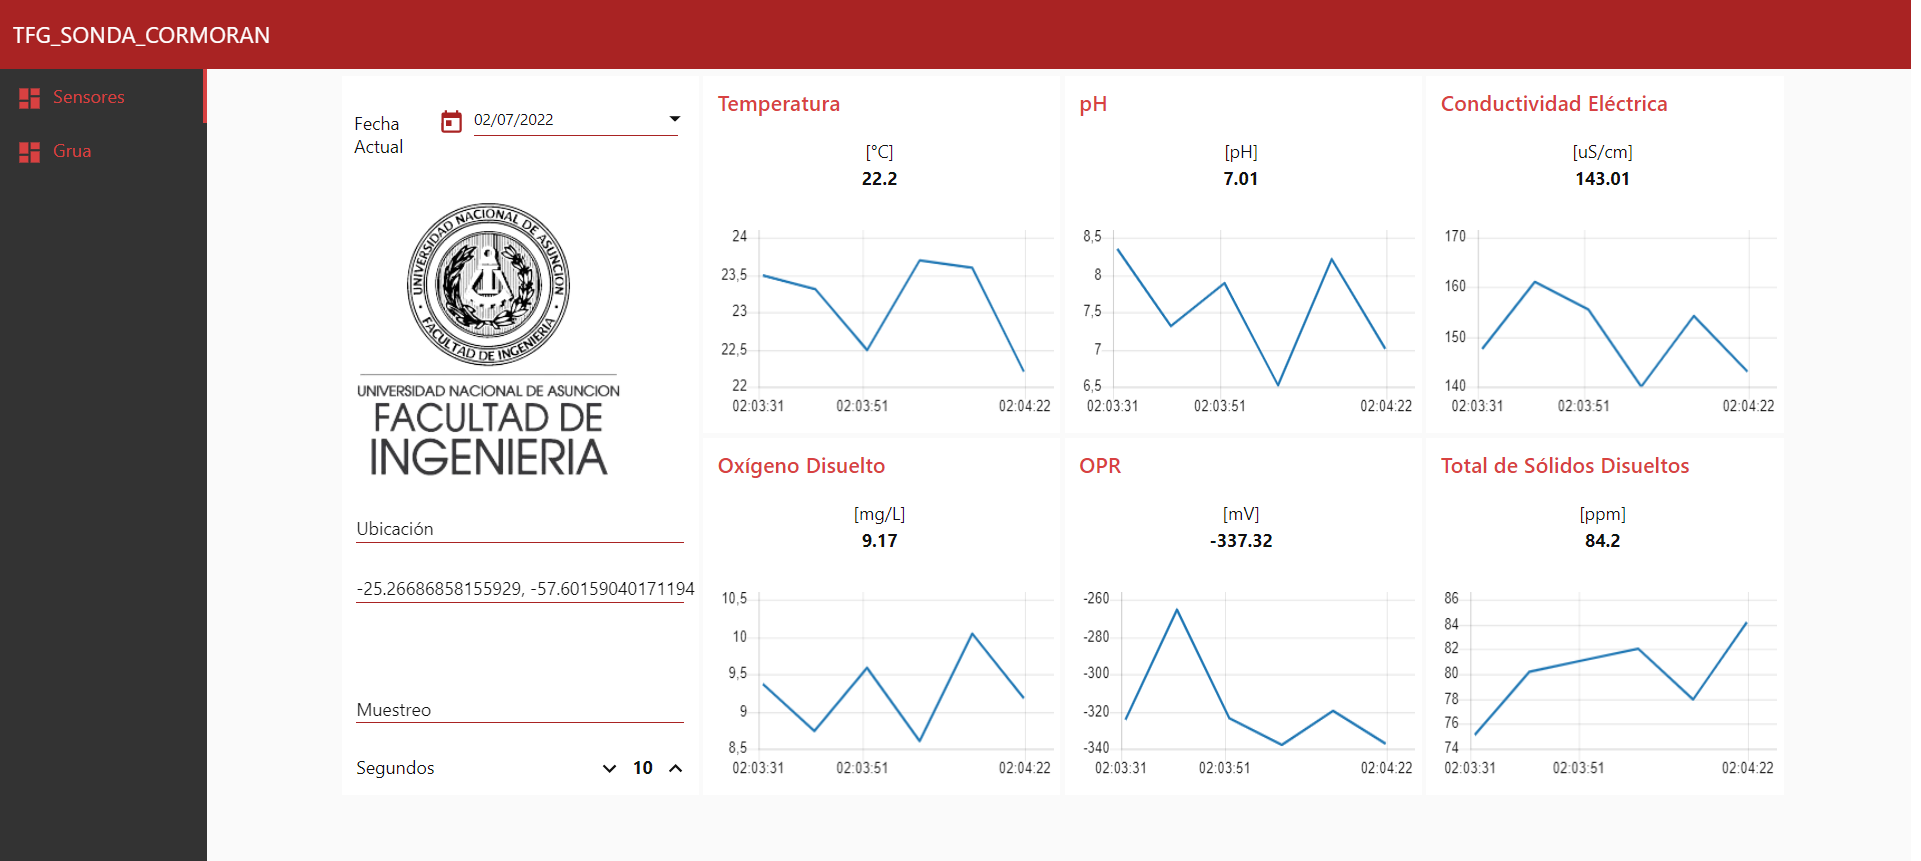
\includegraphics[scale=0.88]{Imagenes/cap4/nodeRed.png}
        \caption {Interfaz de monitoreo. }{\textbf{Fuente:}
        Elaboraci\'on Propia. }
        \label{fig:interfaz}
\end{figure}

Con la idea de conservar un dise\~no m\'inimo, se desarrollaron dos vistas principales. La primera vista, donde se pueda visualizar los datos recolectados por los sensores y otra vista para operaciones manuales. En la figura \ref{fig:interfaz} se puede apreciar el panel principal del monitoreo, donde se despliegan cada uno de los parámetros de temperatura, potencial de hidrógeno, conductividad eléctrica, oxigeno disuelto, potencial de oxigeno reducción y total de solidos disueltos, con gráficos obtenido de la representacion  con cada uno de los puntos obtenidos durante el muestreo de de la la sonda. Además se despliegan las informaci\'ones de la fecha, ubicación en coordenadas de latitud y longitud, del lugar donde se esta obteniendo cada una de las muestras.
\section[Presupuesto]{Presupuesto}
En la Tabla \ref{tab:presu} se puede apreciar los materiales utilizados en el presente TFG y los costos de los mismos.

\begin{table}[t]
\protect\caption{Presupuesto Final del TFG.}
     \label{tab:presu}
     \centering
\begin{tabular}{c l c c}
\hline
\multicolumn{4}{c}{\textbf{Parte mecánica}}\\ 
% \hline
\multicolumn{1}{c}{\textbf{Cant}}                 & 
\multicolumn{1}{c}{\textbf{Descripción}}           & 
\multicolumn{1}{c}{\textbf{Costo USD}}             & 
\multicolumn{1}{c}{\textbf{Total USD}} \\ 
\hline
\multicolumn{2}{l}{\textbf{Sonda}}                & 
\multicolumn{2}{l}{} \\ 
\hline
\multicolumn{1}{c}{1}                             & 
\multicolumn{1}{l}{Cilindro teflón sólido l x D 42x12 {[}cm {]}}        & 
\multicolumn{1}{r}{120,00}                            & 
\multicolumn{1}{r}{120,00}                \\ 
% \hline
\multicolumn{1}{c}{1}                             & 
\multicolumn{1}{l}{Soporte metálico}               & 
\multicolumn{1}{r}{5,00}                              & 
\multicolumn{1}{r}{5,00}                  \\ 
\multicolumn{1}{c}{1}                             & 
\multicolumn{1}{l}{Mecanizado}               & 
\multicolumn{1}{r}{100,00}                              & 
\multicolumn{1}{r}{100,00}                  \\ 
% \hline \\
\multicolumn{2}{l}{\textbf{Periféricos}}          & 
\multicolumn{2}{c}{}                                                             \\ 
\hline
\multicolumn{1}{c}{5}                              & 
\multicolumn{1}{l}{Caño PVC 3/8 pulg.}             & 
\multicolumn{1}{r}{2,00}                              & 
\multicolumn{1}{r}{10,00}                 \\ 
% \hline
\multicolumn{1}{c}{1}                             & 
\multicolumn{1}{l}{Soporte grúa}                   & 
\multicolumn{1}{r}{5,00}                              & 
\multicolumn{1}{r}{5,00}                  \\ 
% \hline
\multicolumn{2}{r}{\textbf{Total parte mecánica}} & 
\multicolumn{2}{r}{\textbf{USD 240,00}}                                             \\ 
\hline                                              &                                                                                                          &                                                                                                          &                                         \\  \\ 
\hline
\multicolumn{4}{c}{\textbf{Parte electrónica}}  \\
% \hline
\multicolumn{1}{r}{\textbf{Cant}}                 & 
\multicolumn{1}{c}{\textbf{Descripción}}           & 
\multicolumn{1}{c}{\textbf{Costo USD}}             & 
\multicolumn{1}{c}{\textbf{Total USD}} \\ 
\hline
\multicolumn{2}{l}{\textbf{Sonda}}                & 
\multicolumn{2}{c}{}                                                             \\ 
\hline
\multicolumn{1}{c}{1}                             & 
\multicolumn{1}{l}{Sensor pH de Atlas Scientific}  & 
\multicolumn{1}{r}{74,99}                          & 
\multicolumn{1}{r}{74,99}              \\ 
% \hline
\multicolumn{1}{c}{1}                             & 
\multicolumn{1}{l}{Sensor conductividad eléctrica Atlas Scient.} & 
\multicolumn{1}{r}{157,99}                         & 
\multicolumn{1}{r}{157,99}             \\ 
% \hline
\multicolumn{1}{c}{1}                             & 
\multicolumn{1}{l}{Sensor oxigeno disuelto de Atlas Scientific}    & 
\multicolumn{1}{r}{217,99}                         & 
\multicolumn{1}{r}{217,99}             \\ 
% \hline
\multicolumn{1}{c}{1}                             & 
\multicolumn{1}{l}{Sensor OPR de Atlas Scientific} & 
\multicolumn{1}{r}{114,99}                         & 
\multicolumn{1}{r}{114,99}             \\ 
% \hline
\multicolumn{1}{c}{1}                             & 
\multicolumn{1}{l}{Sensor temperatura}             & 
\multicolumn{1}{r}{11,95}                          & 
\multicolumn{1}{r}{11,95}              \\ 
% \hline
\multicolumn{1}{c}{1}                             & 
\multicolumn{1}{l}{Kit Raspberry pi 3 B+}          & 
\multicolumn{1}{r}{74,99}                          & 
\multicolumn{1}{r}{74,99}              \\ 
% \hline
\multicolumn{1}{c}{1}                             & 
\multicolumn{1}{l}{Tentacle Shield}                & 
\multicolumn{1}{r}{126,99}                         & 
\multicolumn{1}{r}{126,99}             \\ 
% \hline
\multicolumn{1}{c}{1}                             & 
\multicolumn{1}{l}{Driver pH de Atlas Scient.}     & 
\multicolumn{1}{r}{39,99}                          & 
\multicolumn{1}{r}{39,99}              \\ 
% \hline
\multicolumn{1}{c}{1}                             & 
\multicolumn{1}{l}{Driver conductividad eléctrica Atlas Scient.} & 
\multicolumn{1}{r}{59,99}                          & 
\multicolumn{1}{r}{59,99}              \\ 
% \hline
\multicolumn{1}{c}{1}                             & 
\multicolumn{1}{l}{Driver oxígeno disuelto de Atlas Scient.}        & 
\multicolumn{1}{r}{45,99}                          & 
\multicolumn{1}{r}{45,99}              \\ 
% \hline
\multicolumn{1}{c}{1}                             & 
\multicolumn{1}{l}{Driver OPR de Atlas Scientific} & 
\multicolumn{1}{r}{39,99}                          & 
\multicolumn{1}{r}{39,99}              \\ 
% \hline
\multicolumn{1}{c}{1}                             & 
\multicolumn{1}{l}{Batería LiPo nano-tech 5100mAh} & 
\multicolumn{1}{r}{41,93}                          & 
\multicolumn{1}{r}{41,93}              \\ 
% \hline
\multicolumn{1}{c}{1}                             & 
\multicolumn{1}{l}{Conversor DC-DC}                & 
\multicolumn{1}{r}{10,00}                             & 
\multicolumn{1}{r}{10,00}                 \\ 
% \hline
\multicolumn{1}{c}{1}                             & 
\multicolumn{1}{l}{PCB}                            & 
\multicolumn{1}{r}{20,00}                             &
\multicolumn{1}{r}{20,00}                 \\ 
% \hline\\
\multicolumn{2}{l}{\textbf{Periféricos}}          &
\multicolumn{2}{l}{}                                                             \\ 
\hline
\multicolumn{1}{c}{2}                             & 
\multicolumn{1}{l}{NodeMCU}                        & 
\multicolumn{1}{r}{12,00}                             & 
\multicolumn{1}{r}{24,00}                 \\ 
% \hline
\multicolumn{1}{c}{1}                             & 
\multicolumn{1}{l}{Sonar ultrasónico}              & 
\multicolumn{1}{r}{89,95}                          & 
\multicolumn{1}{r}{89,95}              \\ 
% \hline
\multicolumn{1}{c}{4}                             & 
\multicolumn{1}{l}{Bateria Ion litio 2000mAh}      & 
\multicolumn{1}{r}{12,95}                          & 
\multicolumn{1}{r}{51,8}               \\ 
% \hline
\multicolumn{1}{c}{1}                             & 
\multicolumn{1}{l}{Cabrestante eléctrico}          & 
\multicolumn{1}{r}{119,75}                         & 
\multicolumn{1}{r}{119,75}             \\ 
% \hline
\multicolumn{1}{c}{1}                             & 
\multicolumn{1}{l}{Driver de motor bidireccional}  & 
\multicolumn{1}{r}{29,99}                          & 
\multicolumn{1}{r}{29,99}              \\ 
\hline 
\multicolumn{2}{r}{\textbf{Total parte electrónica }}  & 
\multicolumn{2}{r}{\textbf{USD 1.353,27}}   \\ 
% \hline
\multicolumn{2}{r}{\textbf{Mano de obra}}         & 
\multicolumn{2}{r}{\textbf{ USD 2.200,00}}      \\ 
% \hline
\multicolumn{2}{r}{\textbf{Total genera}}        & 
\multicolumn{2}{r}{\textbf{USD 3.793,27}}  \\ 
\hline
\end{tabular}
\end{table}